\section{Representation Regularization in TD-Learning}
\label{sec:problem}

% Deep RL algorithms can be unstable
Deep RL algorithms suffer from a number of optimization challenges. For example, a simple choice such as the number of gradient steps can have drastic effect on the results~\citep{fedus2020revisiting, fu2019diagnosing}: too few gradient steps will give rise to underfitted Q-functions, but perhaps surprisingly, too many gradient steps can also lead to poor performance (Figure~\ref{fig:atari_5_percent}, Figure 2 in \citep{kumar2021implicit}, Figure 15 in \citep{fu2019diagnosing}). A simple explanation for this phenomenon is that more gradient steps lead to more backups from out-of-distribution actions~\citep{kumar19bear} giving rise to erroneously over-optimistic Q-values. However, while offline RL methods that prevent overestimation in the backup~\citep{wu2019behavior,kumar2020conservative} are considerably more stable than na\"ve value-based RL methods, even these methods often suffer form instability when trained for long~\citep{kumar2021implicit}.  

%%AK: Should we put a figure showing the performance going up and down trend here, or just appeal to learning curves that appear later in the paper and in other papers?
%%SL.5.22: Given the revisions to the previous paragraph, starting with "While this phenomenon might resemble statistical overfitting" seems awkward...
While this phenomenon might resemble statistical overfitting at first glance, as we will show, it is actually a form of underfitting caused by excessive implicit regularization that results from training deep networks with bootstrapping, which is exacerbated in the presence of out-of-distribution actions. As we will show, this implicit regularization causes the network to ``co-adapt'' representations on the state-action tuples appearing on two sides of the Bellman update, making such Q-functions less able to distinguish dataset actions from the actions of the current policy. This is highly problematic, since the whole point is to learn a policy that takes better actions than the ones in the dataset.
%%SL.5.22: I tried to expand on the above a bit, feel free to revert though if this doesn't make sense.
We will first provide empirical evidence of this co-adaptation phenomenon. Then, under an idealized model of neural network training~\citep{wei2019regularization,savarese2019infinite}, we will show theoretically how this co-adaptation phenomenon arises. Finally, we will discuss the adverse consequences of this co-adaptation phenomenon and devise a method to address it by introducing \emph{explicit} regularization.

\subsection{An Empirical Observation: Feature Co-Adaptation in TD-Learning}
\begin{wrapfigure}{r}{0.42\textwidth}
    \centering
    \vspace{-15pt}
    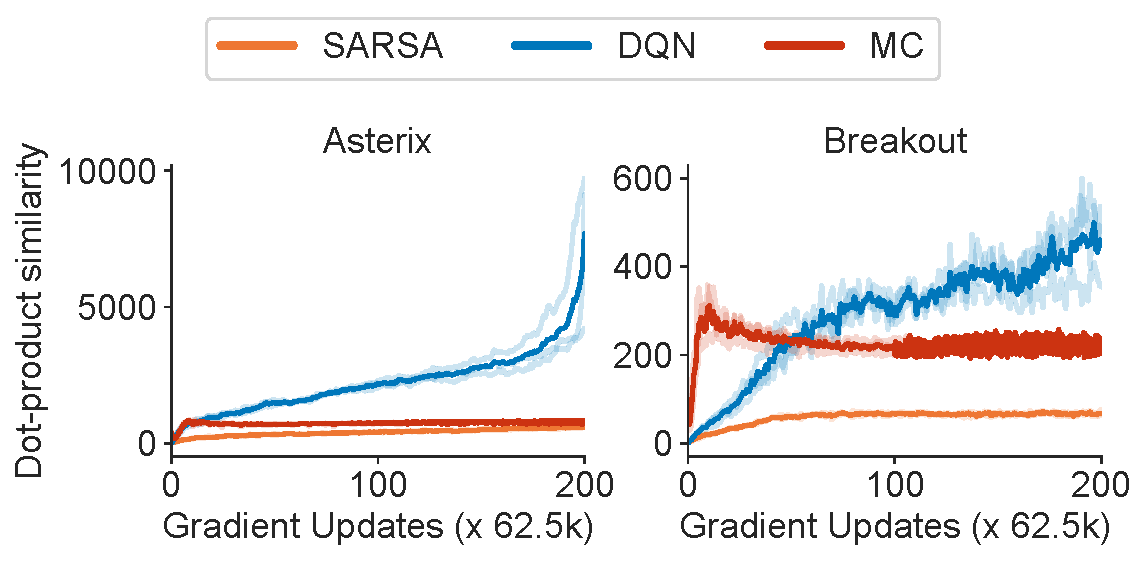
\includegraphics[width=0.97\linewidth]{section3_figs/figure1_dotproduct_dot_products.pdf}\\
    ~~~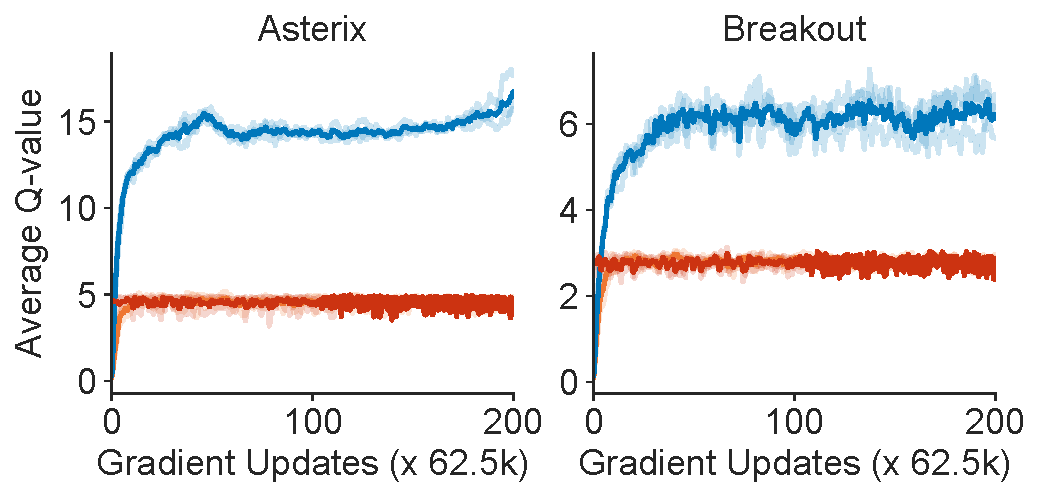
\includegraphics[width=0.94\linewidth]{section3_figs/figure1_dotproduct_q_values (1).pdf}
    \vspace{-0.24cm}
    %%SL.5.22: Let's not label it "MC", that's not very informative. Call it "supervised" instead.
    \caption{\small{Dot-product $\Delta(\bs, \ba, \bs', \ba')$ increases through training for DQN even though the average Q-value stays relatively constant, while SARSA and MC exhibit near-constant dot product similarities as well.}}  
    \label{fig:dot_products}
    \vspace{-0.4cm}
\end{wrapfigure}
%%AK: I thought about this a bit, but it was not clear how to best describe why we tried this experiment, so I just started by describing this phenomenon. Any suggestions for restructuring would be appreciated.
We start our analysis with an empirical observation regarding the last-layer features learned by a deep network trained via Q-learning in the offline RL setting.
%%SL.5.22: Can we set this up with more details about what this is showing? Offline or online? Is it just grad steps, or also flipping the target network? Is it evaluation or maximization? Also, isn't this unsurprising, since DQN does not protect against OOD actions? Without these details, readers won't really appreciate this, and will just say it's obvious.
As shown in Figure~\ref{fig:dot_products}, as we take more gradient steps via Bellman backups, the dot product similarity between the features learned by the Q-function at 
state-action pairs $(\bs, \ba)$ and $(\bs', \ba')$ that appear together in a Bellman backup, denoted by $\Delta(\bs, \ba, \bs', \ba') := \phi(\bs, \ba)^\top \phi(\bs', \ba')$
%%SL.5.22: Delta typically indicates change, let's use a different symbol.
continually increases. We evaluate three methods: DQN~\citep{Mnih2015}, which potentially uses out-of-distribution $(\bs', \ba')$ for the backup, supervised regression to Monte-Carlo returns (MC), and SARSA, which uses $(\bs', \ba') \in \mathcal{D}$ for computing target values. While the value of $\Delta$ steadily increases for DQN over time, $\Delta$ remains relatively flat for supervised regression and SARSA. Note that the Q-values learned by DQN do not actually exhibit overestimation, as shown in ???.
%%SL.5.22: Overall, I think if I read this paragraph for the first time, I would think this was either obvious or highly questionable. DQN is solving a completely different from SARSA and regression, so it shouldn't be surprising that it learns different features. It's also not "supposed" to work because of OOD actions. Furthermore, the plot doesn't appear to show that anything bad actually happens. So what's the big deal? I think perhaps more setup is needed to make this example palatable to the reader. I think we need to set this up more slowly, discuss how supervised regression leads to stable features, while the dot products of features learned with DQN grown over time, and are much larger overall. This is surprising, because both methods are trying to learn the same Q-function, so if DQN was converging to the correct Q-function (the one that the MC method is regressing to), we would expect it to come up with similar features. We might also want to mention that larger dot products may indicate that the features are becoming more similar to each other (this may not be obvious)

Why does performance degrade in Q-learning even though the amount of overestimation in Q-values does not significantly change? Is the unusual trend in the feature dot products related to this in some way? We will show in Section~\ref{sec:analysis} that the growth in the value of $\Delta(\bs, \ba, \bs', \ba') = \phi(\bs, \ba)^\top \phi(\bs', \ba')$ is a direct consequence of the implicit regularization induced by gradient descent when combined with TD updates. When DQN bootstraps from $(\bs', \ba') \notin \mathcal{D}$, the implicit regularization phenomenon adapts otherwise unconstrained
%%SL.5.22: what does unconstrained mean?
features, $\phi(\bs', \ba')$, to minimize the implicit regularizer.
%%SL.5.22: what implicit regularizer? let's not throw around this term so loosely without having defined it. I also think that perhaps that entire sentence could be removed or replaced with something very brief.
Thus the learned network features may simply minimize TD error, but may not attain a valid Q-function.
%%SL.5.22: This sounds silly -- minimizing TD error generally means attaining a valid Q-function. If you want to say something like this, you need to *very* clearly explain why these would be different.
We refer to this phenomenon as ``co-adaptation'' between features at $(\bs, \ba)$ and $(\bs', \ba')$ and it produces highly similar features at these tuples. Such a co-adaptation is undesirable because it couples the values at seen and unseen actions, which is expected to give poor policy performance. Such a phenomenon can be avoided by using SARSA.  
%%SL.5.22: My recommendation would be not to fixate on SARSA so much. It's a distraction.

% In what follows, we will show that the increased dot-product similarities at $\phi(\bs, \ba)$ and $\phi(\bs', \ba')$ is a direct consequence of the phenomenon that when features at $\phi(\bs', \ba')$ are not explicitly controlled via the data distribution (e.g., when $(\bs', \ba') \notin \mathcal{D}$), implicit regularization of gradient descent on the Q-network would encourage the network to learn representations $\phi(\bs', \ba')$ that alias with $\phi(\bs, \ba)$ as this is a favorable strategy for optimizing the implicit regularizer. Purely supervised methods that do not use bootstrapping or methods that use on-policy bootstrapping, \ie $(\bs', \ba') \in \mathcal{D}$ (e.g., SARSA) do not suffer from this issue.    

\subsection{Theoretical Analysis of Feature Co-Adaptation in TD-Learning}

In this section, we present theoretical analysis of how the features learned via TD-learning differ from the features learned via standard supervised deep learning, which will shed light on the peculiar phenomena observed empirically in the previous section.
%Having observed the differences in feature evolution in Q-learning and in supervised regression in terms of high dot-products between features, and the disconnect from overestimation in Q-values, we now theoretically establish how implicit regularization induces feature co-adaptation, leading to a form of feature aliasing between representations at $(\bs, \ba)$ and $(\bs', \ba')$.


% In standard supervised learning, overparameterized neural networks can learn without massive overfitting, even when provided with very few datapoints compared to the number of parameters of the network. While the success of overparameterization has partly been explained via the implicit regularization effect of gradient descent on such large models~\citep{arora2018optimization,arora2019implicit,gunasekar2017implicit,gunasekar2018implicit}, it is less clear how it affects TD-learning algorithms. In particular, we ask the following questions: how are representations learned by overparameterized networks in TD-learning different from those learned in supervised learning? Is the implicit regularization effect of large network training beneficial in TD-learning? 

% Since representation regularization in supervised learning possess favorable properties~\citep{arora2018optimization,arora2019implicit},
%%SL.5.17: I think we need to ease the reader into it. Don't assume they are an expert, start with something like: Overparameterized neural networks often have many more parameters than the number of datapoints they are trained on. This poses a puzzle for machine learning theory: why do large neural networks not suffer more heavily from overfitting? Why do the solutions learned with deep learning generalize well? A number of recent works have proposed various \emph{implicit} regularization mechanisms...
%%AK: addressed
% we first ask the question: how are representations learned by neural networks in TD-learning different from those learned via supervised learning? A direct comparison will help us analyze the consequences of the regularization effects in these cases. 

%%SL.5.17: We start using a bunch of terminology (e.g., \Phi, w) in this section that is not actually introduced in the preliminaries -- perhaps it would help to give a short 1-paragraph crash course on min-norm stuff in preliminaries, to make it more natural to tie it in here?

%%AK: maybe I can define some basics in prelims?
Since the full learning dynamics involved in neural network training are complex and difficult to analyze exactly, prior works typically analyze more idealized problems that provide a reasonable model for the behavior of deep learning with stochastic gradient descent. One widely studied surrogate is the min-norm interpolant~\citep{hastie2019surprises}.
%%SL.5.22: I think we need more details to explain and justify this. In particular, readers unfamiliar with this idea will not understand whether this is just a problem that we are *postulating* is similar (which of course is silly to do without evidence), or if prior work has shown (theoretically or empirically) that this formulation is a reasonable model of what deep learning actually does. Basically, we need to support (with citations) the statement that this min-norm program is a good model for the behavior of representation learning with deep nets. The current phrasing does not do that.
Following this paradigm, we can reformulate TD learning and supervised learning as effectively training a linear regression model on a large number of feature transforms of the input~\citep{wei2019regularization,savarese2019infinite}, where the implicit regularization effect encourages weight-vectors that have the minimal $\ell_1$ norm -- \ie, weight vectors that effectively utilize the least number of features for fitting the data. An example of such an optimization problem for supervised regression to Q-values is shown in Equation~\ref{eqn:min_norm} (right). Following prior work~\citep{wei2019regularization}, the feature transforms
%%SL.5.22: "transforms"?
$\Phi$ are typically given by ReLU features, such that $\Phi_{\bs, \ba} = [\cdots, (\bu_i^T (\bs, \ba))_{+}, \cdots]$, where $\bu_i \sim \mathcal{N}(0, \bI)$.
%%SL.5.22: what is the significance of u? does this show up anywhere else? is it needed?
By deriving and analyzing the TD-solution under this framework, and contrasting it with supervised regression, we aim to build an understanding of how implicit regularization affects TD-learning.
%%SL.5.22: There is some repetition between the above paragraph and the paragraph below in presenting the min-norm formulation. But I think the paragraph below does it quite a bit better, because it first presents the supervised version, and then extends it to the TD version, while the above paragraph tries to present it all at the same time, which is quite confusing.

%%AK: need to define relu features properly in prelims
\textbf{Min-norm TD solution.} Prior works provide a form for the min-norm problem for supervised regression (Equation~\ref{eqn:min_norm}, right). Our analysis of TD learning starts by deriving the corresponding min-norm optimization problem for the TD-fixed point. TD-learning can be modelled as solving a sequence of supervised regression problems (\ie fitted Q-iteration~\citep{Riedmiller2005}), each one regressing onto targets generated from the previous Q-function. The final TD-fixed point (denoted as $\bw^*$) can however still be expressed as the minimal $\ell_1$ norm weight vector $\bw^*$ of a single optimization problem that attains Bellman consistency for all transitions $(\bs, \ba, \bs', \ba') \in \mathcal{D}$, projected onto the feature map $\Phi$. We formally derive this problem for TD-learning using techniques from LSTD~\citep{lagoudakis2003least} in Appendix ??. The resulting min-norm optimization problem for TD-learning is given below (Equation~\ref{eqn:min_norm}, left):
%%SL.5.22: Something here that will be very confusing to readers who are not super familiar with this sort of analysis is that this is overparameterized. If it were not overparameterized, this would not be a valid way to write linear regression. Can you just add a sentence somewhere in the above para or the previous one to make this clear? It can be a very brief remark (e.g., in the overparameterized regime, $\bw$ can admit multiple different solutions, all of which fit the data equally well...
%%SL.5.22: Additionally, it is left rather ambiguous above if we are still talking about last layer features, or NTK, or something else. Most readers will assume we mean last layer features, but those are *not* overparameterized, making this really confusing.
\begin{equation}
\begin{aligned}
    &\text{\textbf{TD-learning}} \\
    \min_{\bw, \Phi}~~& ||\bw||_1 \\
    \text{s.t.}~~&~ {\Phi}^\top {\Phi} \bw = {\Phi}^\top R + \gamma {\Phi}^\top \left(\hat{P}^\pi \Phi \right) \bw
\end{aligned}
%%AK: the prelims section will go into why linear TD can be written as the constraints here
\;~~~~~ \vline\;
\begin{aligned}
    &\text{\textbf{Supervised regression}} \\
    ~~~~~~~\min_{\bw, \Phi}~~& ||\bw||_1 \\
    \text{s.t.}~~&~ {\Phi} \bw = Q^\pi % := {\Phi}^\top (I - \gamma P^\pi)^{-1} R
\end{aligned}
%%AK: should we write this in a per-datapoint form and not in matrix form?
%%SL.5.17: err what?? the equation on the right is *not* supervised learning!
%%AK: Sorry I am not sure I follow -- isn't this supervised regression to Q^\pi? What else should we compare to? 
\label{eqn:min_norm}
\end{equation}
Since Equation~\ref{eqn:min_norm} presents linear regression problems over $\bw$, we can express the optimal $\bw^*$ in terms of the corresponding optimal learned features, $\Phi^*$, as a solution to a Lasso regression problem~\citep{hastie2015sparsity}:
%%SL.5.22: Don't sweep under the rug the difference between an inverse and a pseudoinverse! The inverse doesn't make sense for overparameterized problems, and Equation 1 doesn't make sense for problems that are not overparameterized, so either Eq 1 is wrong, or Eq 2/3 is wrong. Just introduce a symbol for pseudoinverse and explain why it leads to the min norm solution.
\begin{align}
    \bw^*_{\mathrm{TD}} ~&= \left[\Phi_{\mathrm{TD}}^\top \left(\Phi_{\mathrm{TD}} - \gamma \left(\hat{P}^\pi \Phi_{\mathrm{TD}} \right) \right)\right]^{-1} \left( \Phi_{\mathrm{TD}}^\top R - \bz_\mathrm{TD} \right),  \label{eqn:td_soln} \\
    \bw^*_{\mathrm{Sup}} ~&= \left[\Phi_{\mathrm{Sup}}^\top \Phi_{\mathrm{Sup}}\right]^{-1} \left(\Phi_{\mathrm{Sup}}^\top Q^\pi - \bz_{\mathrm{Sup}}\right)  \label{eqn:sup_soln},
\end{align}
where $\bz_\mathrm{TD}$ and $\bz_{\mathrm{Sup}}$ denote the induced offsets in Lasso.
%%SL.5.22: citation?
These offsets threshold small,
%%SL.5.22: something is malformed in this sentence
but non-zero entries of $\bw^*$ to 0~\citep{hastie2015sparsity}, thereby sparsifying $\bw^*$. These offsets are bounded elementwise, and we leave further technical details to Appendix ??.  
%%SL.5.22: This may be an unsolvable problem, but I found this discussion of offsets and l1 incredibly confusing, perhaps because it so terse.

\textbf{Difference between $\bw^*_{\mathrm{TD}}$ and $\bw^*_{\mathrm{Sup}}$.} Perhaps the most striking difference between the TD and supervised learning solutions in Equations~\ref{eqn:td_soln} and \ref{eqn:sup_soln} is the presence of a a term dependent on the \emph{learned} features $\hat{P}^\pi \Phi$ (i.e., $\phi(\bs', \ba')$) computed at $(\bs', \ba')$, which can potentially be out of the training distribution, appearing on the right-hand side of the constraint in TD-learning optimization problem, whereas supervised learning only utilizes the features $\phi(\bs, \ba) \in \mathcal{D}$.
%%SL.5.22: The reader will have no idea what \hat{P}^\pi \Phi_TD is because it was never defined, so they will not find this striking. That's because \hat{P}^\pi \Phi_TD is not correct notation. The next step features are not a linear transformation of dataset features, they are just different features, and should be written as such. E.g., \Phi'. But if you write it like that, you need to clearly define what they mean in the text *before* Equation 1.
How does this difference affect the resulting solution, especially since all of these feature vectors $\Phi$ are learned?  
%%SL.5.22: I'm not sure asking this question here is productive. It would be better here to present the argument more top-down rather than bottom up, otherwise you just have too many steps of indirection and too many things the reader needs to keep in their head. It's OK to briefly mention that you have these \Phi' features, but don't pose this question -- you've posed too many questions already without answering them. The structure should not be question question question answer answer answer, but question answer question answer question answer, otherwise the paper is just too difficult to read. So what I suggest is: cut this paragraph, replace it with a brief 1-sentence remark about Phi', and proceed with the main argument.

\textbf{Feature are co-adapted.} Consider an extreme scenario where $(\bs', \ba') \notin \mathcal{D}$ for any transition $(\bs, \ba, \bs') \in \mathcal{D}$. In this case, additional reduction in $||\bw||_1$ can be obtained by specifically setting the values of $\phi(\bs', \ba')$ so as to ensure a complete cancellation of information across certain feature dimensions unnecessary to predict the reward function,
%%SL.5.22: too vague ("cancellation of information across certain feature dimensions unnecessary to predict the reward function")
thereby leading to a more sparse $\bw^*_{\mathrm{TD}}$. While this may be enough to minimize TD error, such feature vectors may not be predictive of the overall long-term Q-function. This is what we call \emph{feature co-adaptation}: by setting values of features $\phi(\bs', \ba')$ at unseen $(\bs', \ba')$ in special ways relative to $\phi(\bs, \ba)$, TD-learning can recover overly regularized (i.e., smaller $||\bw||_1$) solutions which may not be able to express the groundtruth value functions. 
%%SL.5.22: I think this paragraph is too hand-wavy right now.

We formalize this basic insight and more generally show that even when TD-learning backs up from only one out-of-distribution point $(\bs', \ba')$, the resulting solution $\bw^*_{\mathrm{TD}}$ is more sparse if learned features $\phi(\bs, \ba)$ and $\phi(\bs', \ba')$ are similar to each other. This leads to a drop in the rank of $\bM_{\mathrm{TD}}(\Phi) = \Phi_{\mathrm{TD}}^\top (\Phi_{\mathrm{TD}} - \gamma (\hat{P}^\pi \Phi_{\mathrm{TD}}))$ and increased dot-products $\phi(\bs, \ba)^\top \phi(\bs', \ba')$, thus explaining the trends from Figure~\ref{fig:dot_products}. We present our result informally below, and defer the complete theorem statement and a proof to Appendix ??.
\begin{theorem}[Informal]
\label{thm:aliasing_exists}
Let $\Phi_{\mathrm{TD}}$, $\Phi_{\mathrm{Sup}}$, $\bw^*_{\mathrm{TD}}$ and $\bw^*_{\mathrm{Sup}}$ denote solutions to Equation~\ref{eqn:min_norm}. Let the supervised solution, $\Phi_{\mathrm{Sup}}$ satisfy: $\mathrm{srank}\left(\bM_{\mathrm{Sup}}(\phi^*)\right) = r_0$. Then, even when using only one unseen $(\bs', \ba')$ in the backup, the effective expressivity of the TD solution decreases: $\mathrm{srank} \left(\bM_{\mathrm{TD}}(\phi^*)\right) < r_0$.
\end{theorem}
Theorem~\ref{thm:aliasing_exists} implies that even in cases where supervised regression to the groundtruth $Q^\pi$ (or $Q^*$) requires at least rank-$r_0$ features, feature co-adaptation in TD-learning can potentially reduce the effective rank of $\Phi$ learned below this value, crippling the ability of the Q-function to represent the actual function despite being (vastly) overparameterized. 

\begin{wrapfigure}{r}{0.47\textwidth}
    \centering
    \vspace{-10pt}
    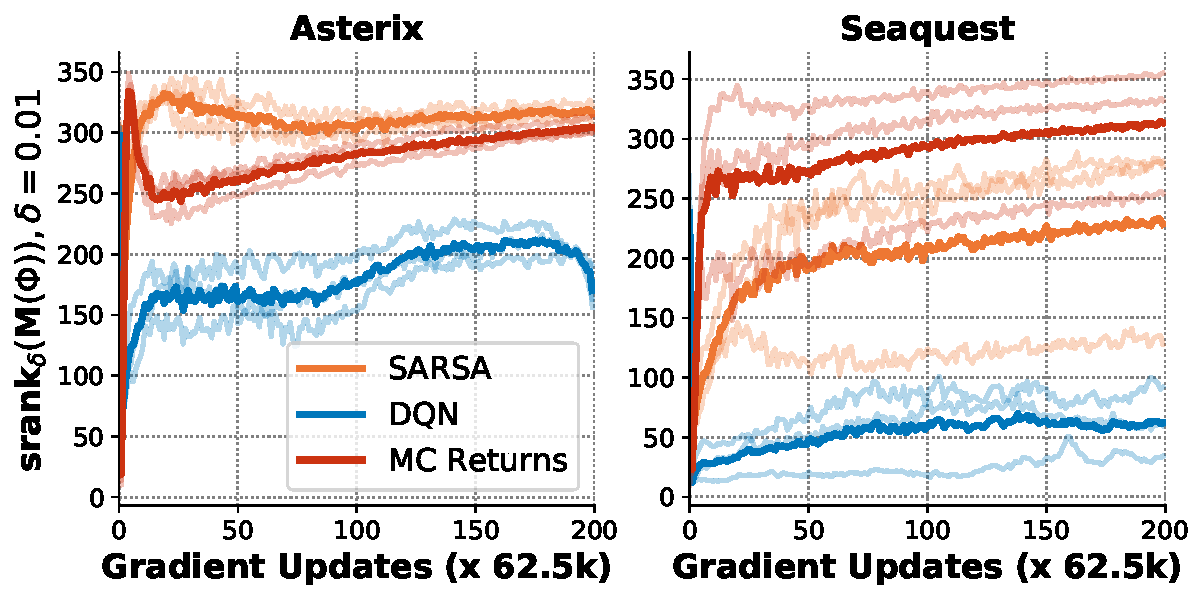
\includegraphics[width=0.97\linewidth]{section3_figs/srank_sarsa_vs_mc_vs_dqn_fig1_only_main_paper.pdf}
    \vspace{-0.14cm}
    \caption{\small{Effective ranks of $\bM(\phi)$ for DQN, SARSA and MC returns. Note that DQN indices the least rank matrix M, while SARSA and MC induce similar rank $\bM(\phi)$, thus validating Theorem~\ref{thm:aliasing_exists}.}}
    \label{fig:srank}
    \vspace{-0.4cm}
\end{wrapfigure}
While Theorem~\ref{thm:aliasing_exists} is related to Theorem 4.1 in \citep{kumar2021implicit} in the high-level motivation that bootstrapping leads to some sort of aliasing, our result is stronger in that it not only shows that TD-learning produces overly regularized features, but also identifies the cause behind this issue -- using unseen state-action pairs for the backup allows the features at such transitions to co-adapt to each other, allowing them to minimize the TD error without actually recovering a valid Q-function.
%%SL.5.22: that's reasonable, but then the bit you discuss below this seems exactly the same at a glance to IUP
To empirically validate Theorem~\ref{thm:aliasing_exists}, we measure the effective ranks of $\bM_{\mathrm{TD}}(\phi)$ and $\bM_{\mathrm{Sup}}(\phi)$ in Theorem~\ref{thm:aliasing_exists} on two Atari games, as shown in Figure~\ref{fig:srank}. Note the drop in the rank for DQN vs. supervised regression to Monte-Carlo return estimates. Additionally, when using exactly the action observed in the dataset for Bellman backups in SARSA, the rank drop does not exist, validating our connection to out-of-distribution actions.   

\subsection{Consequences of Feature Co-Adaptation in TD-Learning}
Having seen that TD-learning co-adapts features at unseen actions to features at state-action tuples in the dataset, we now study its consequences. We will show that this co-adaptation can prevent learning high-frequency information in the Q-function crucial for control and destabalize learning, even when initialized in the vicinity of a good solution.

\begin{wrapfigure}{r}{0.4\textwidth}
    \centering
    \vspace{-22pt}
    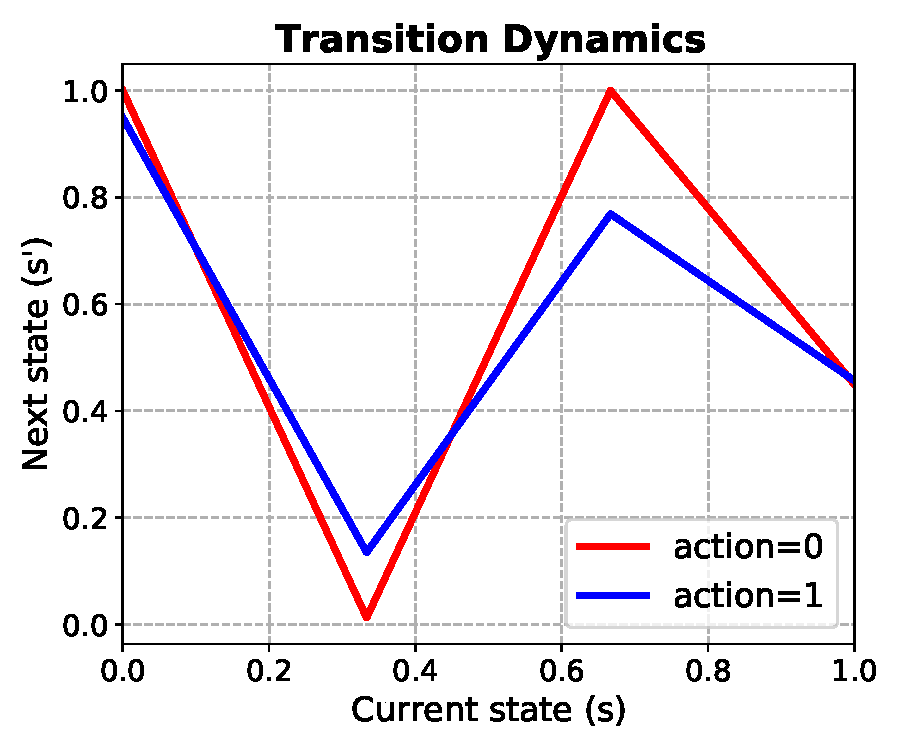
\includegraphics[width=0.48\linewidth]{section3_figs/dynamics.pdf}
    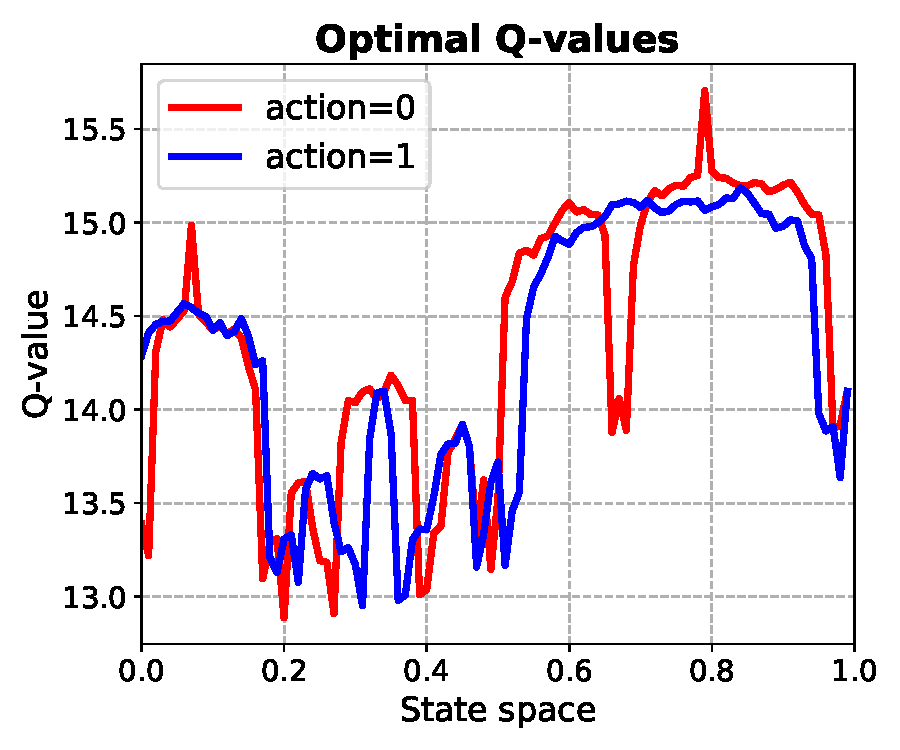
\includegraphics[width=0.48\linewidth]{section3_figs/optimal_q.pdf}
    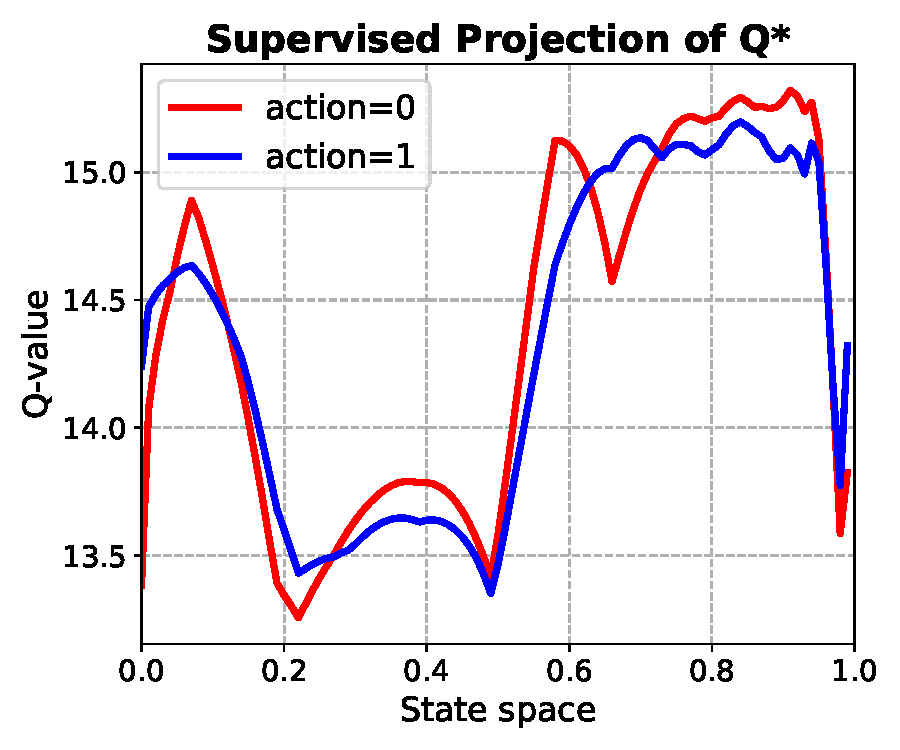
\includegraphics[width=0.48\linewidth]{section3_figs/supervised_q.pdf}
    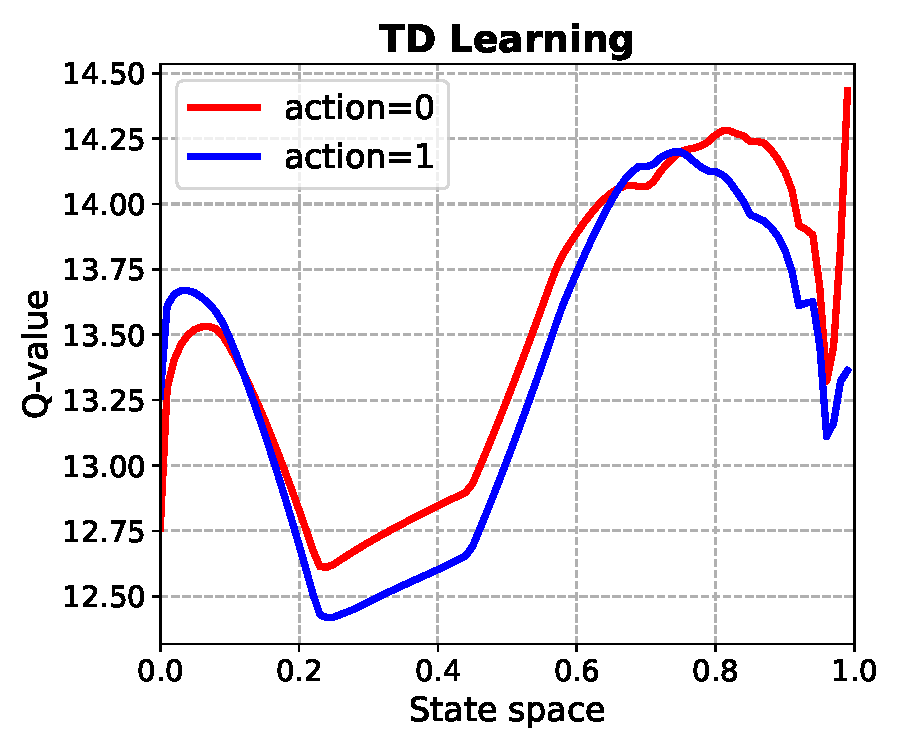
\includegraphics[width=0.48\linewidth]{section3_figs/td_learning.pdf}
    \vspace{-0.21cm}
    \caption{\small{\textbf{TD-learning fails to represent high frequency changes in Q-functions much more than supervised learning.} On the 1D MDP (dynamics, top-left), TD learning ignores the high-frequency components of the Q-function leading to worse action selection compared to supervised regression.}} 
    \label{fig:1d_mdp}
    \vspace{-0.6cm}
\end{wrapfigure}
%%AK: Tengyu had an interesting suggestion here: represent the action choices of each function via a shaded interval on the the number line, using blue for a_0 and red for a_1. The number of switches will determine the complexity of the Q-function, and this will show that TD has 4 switches, supervised has 8 and actual has 12 or 13 switches.
\textbf{Inability to model high-frequency components of Q-function.} Prior work has noted that Q-functions can be highly non-smooth even when reward functions and dynamics are relatively simple~\citep{dong2020expressivity}.
%%AK: does gamma models also note something related to complexity of Q vs reward via the discount profile stuff?
Would feature co-adaptation lead the Q-function to ignore certain high-frequency components in the objective?
As a didactic example of this phenomenon, we utilize a 2-action MDP with a 1-D state space $\mathcal{S} \in [0, 1]$ from~\citep{dong2020expressivity}. This MDP exhibits a piecewise linear dynamics (Fig.~\ref{fig:1d_mdp}, top-left) and an identity reward function $r(\bs, \ba) = \bs$ with two actions $\ba \in \{0, 1\}$. The optimal Q-function exhibits high-frequency changes (Fig.~\ref{fig:1d_mdp}, top-right). We find that running Q-learning (Fig.~\ref{fig:1d_mdp}, bottom-right)
attains Q-functions that completely ignore these high-frequency changes. This often makes the resulting policy choose the worse action of the two possible actions. On the contrary, a supervised projection (Fig.~\ref{fig:1d_mdp}, bottom-left) of the Q-function does capture many of these high frequency shifts in the Q-function. To formalize this didactic example, we prove the following result showing that high-frequency components of the Q-function are not modelled as a direct consequence of Theorem~\ref{thm:aliasing_exists}. The proof and a complete statement for Theorem~\ref{thm:num_pieces} can be found in Appendix ??.

%%AK: this will have some conditions on dynamics too, maybe we mention that as a detail in the appendix? But if it is unclear, maybe we should add it here, and explain it here...
\begin{theorem}[Informal]
Assume that the state-space $\mathcal{S}$ of the MDP is given by the 1-D number line, and that the groundtruth Q-function is (approximately) piecewise linear in the state $s$ with $N^*$ pieces. Denote the (approximate) number of linear pieces in a learned infinite-capacity ReLU Q-network via direct supervised regression as $N_{\mathrm{Sup}}$ and via TD-learning as $N_{\mathrm{TD}}$. Then: $N_{\mathrm{TD}} \leq N_{\mathrm{Sup}} \leq N^*$.     
\label{thm:num_pieces}
\end{theorem}
%%AK: In the proof of this theorem, we show this for approximate number of pieces, which is the integral of the second derivative of the function w.rt.t the input over the input space, but I think going into details would just hurt understanding here.

%%AK: I am a little unsure about the following part, in the sense if we should have it or not? This might seem obvious to some extent? 
% \textbf{Severe co-adaptation renders distributional shift corrections ineffective.} To test whether offline RL corrections alleviate feature co-adaptation, we performed a controlled experiment -- we constrained offline RL regularizers to only control the last linear layer of the Q-network, whereas bootstrapping was allowed to train the entire network. While we might expect that offline RL methods may still be effective by adapting the last weight layer to the features, contrary to this expectation, as shown in Figure ??, we find that all such variants (denoted as CQL($\phi$)) perform extremely poorly compared to the complete offline RL method. Further note the inability to minimize the regularizer corresponding to distributional shift and an increased dot-product similarity, $\Delta(\bs, \ba, \bs', \ba')$. This indicates that feature co-adaptation can lead to failure of offline RL methods. \textcolor{red}{add new figure for this}
%%AK: If we do keep this, maybe we should also add some line to justify why offline RL methods are still sensitive -- this is because they are not exactly doing SARSA?

\textbf{Lack of stability near ``good'' Q-function solutions.}
%%SL.5.22: instead of using a vague term like "good" with scare quotes, can we just say optimal? And what does "lack of stability" mean? Maybe just state it directly: Implicit regularization can prevent convergence, even when initializing at an optimal solution. [or something like that]
Finally, we study if co-adaptation of features cause the TD-learning process to diverge away, even when initialized favorably in the vicinity of a good Q-function (e.g., one obtained via supervised regression to MC returns or one obtained via online RL). Running Q-learning from such a favorable initialization eventually produces solutions that perform poorly as shown in Figure ?? below. Moreover, \textcolor{red}{say something about ranks here}. Indeed, in accordance with Theorem~\ref{thm:aliasing_exists}, the feature co-adaption phenomenon drives learning towards solutions with lower $\srank(\bM_{\mathrm{TD}}(\phi))$ values, giving rise to poor performance. \textcolor{red}{add figure, theorem}      

%%SL.5.17: what are Bellman constraints?
% are only enforced approximately (i.e., when the TD error
% %%SL.5.17: was the TD error ever defined?
% is not exactly 0), the implicit regularization towards minimum $||\bw||_2$ norm solutions will lead to the Q-function ignoring high-frequency components. That is, if the true Q-function changes dramatically from one state to the next, low TD-error solutions will fail to represent these changes.
%%SL.5.17: I don't see why the above theorem indicates that this is true
%%AK: add a worst-case theorem as discussed with George today?
%%SL.5.17: maybe we should put this didactic example into a separate \paragraph{} with more setup, instead of presenting this as a kind of footnote -- as-is, I think many people will not really understand it


%%AK: Check if we can take this paper's "peicewise linear theory" and convert it to a policy improvement bound differentiating between TD and supervised, as opposed to just fitting Q*-values?

% \subsection{Consequences of Overly Regularized Representations in TD Learning}
% Having seen aliasing of features on state-action tuples used for bootstrapping emerge as one pathological consequence of overly regularized representations in TD-learning compared to supervised learning, we next ask the following question we study the impact of over-regularization have on the performance of TD-learning. In particular, we ask: do TD-learning algorithms find generalizing and stable optima? To answer these questions, we consider a simple scenario where learning is initialized from a 


% \textbf{Abstract model.} Our abstract model captures feature learning as making a discrete selection among $K$ different feature vector candidates, $\{\Phi_1, \Phi_2, \cdots, \Phi_K\}$, $\Phi_i \in \mathbb{R}^{|\data|\times d}$,
%%SL.5.13: It would be way easier to understand if we could get continuous domains, and then just frame this as an optimization over \Phi (i.e., optimization over \Phi corresponds to selecting the best \Phi \in [some set]), that way we don't have to have this "discrete selection" business and could just say that it's part of the optimization process.
% and then training a linear layer $\bw \in \mathbb{R}^{d}$ to obtain the Q-function.
%%SL.5.13: One way you could phrase is this: Our abstract model of the learning process separates the neural network into two parts: a representation $\Phi$ and a weight vector $\bw \in ...$, such that the full model is given by $\Phi(..)^T \bw$ (i.e., $\bw$ corresponds to the last linear layer). The learning process is framed as a \emph{bilevel} optimization problem, where the weights $\bw$ are chosen subject to a constraint that the learning process chooses the optimal features $\Phi \in [set]$ for $\bw$ (or something like that)
% To mimic the overparameterized nature of neural networks, we assume that we operate in the overparameterized regime with $n < d$.
%%SL.5.13: This is kind of weird -- usually the last layer features are not that high dimensional, but the model parameters are. Are you sure we shouldn't look for some way to "NTK-ify" this? Perhaps a better way to frame this is that we are in the NTK regime where the choice of Phi corresponds to the choice of NTK (i.e., it's not fixed, as is more common in this analysis), while bw corresponds to the neural net parameters? That would justify the overparameterized regime and make this less weird.
% Assume that the initial value of the weight vector $\bw^{(0)} = 0$. We then write out the minimum-norm optimization problem shown below in Equation~\ref{eqn:min_norm} that attains the same solution as the optimal solution found by minimizing training TD error in this model, and characterize the properties of features $\Phi_K^*$ that are selected to obtain the minimum-norm solution. \textcolor{red}{more assumptions?}     
%%SL.5.13: It won't be clear to some people what min-norm has to do with neural net training, can you cite something to justify this?
% \begin{align}
%     \min_{\bw, \boldm_i \in \{0^d, 1^d \}}~~& ||\bw||_2^2 \nonumber\\
%     \text{s.t.}~~&~ \bar{\Phi}^\top \bar{\Phi} \bw = \bar{\Phi}^\top R + \gamma \bar{\Phi}^\top P^\pi \bar{\Phi} \bw, ~~ \bar{\Phi} = \left[\Phi_1, \cdots, \Phi_k\right] \otimes [\boldm_1, \cdots, \boldm_K]
% \label{eqn:min_norm}
% \end{align}
%%SL.5.13: ouch, this \bm_i is... difficult to parse
% Our first result characterizes the feature representation $\bar{\Phi}$ -- equal to one of $\Phi_i$ selected based on the learned masks $\bm_i$ -- that satisfies the Bellman consistency condition but also minimize the implicit regularizer, $||\bw||_2^2$,
% %%SL.5.13: where does this implicit regularizer come from?
% and use this to depict the existence of this phenomenon.


\iffalse

\section{Representation Regularization in Offline Q-Learning}
\label{sec:problem}
%%SL.5.13: See my comment on the title about "excessive" (maybe we call it Implicit Over-Regularization?). That said, this again sounds *extremely* similar to IUP, to the point where the section title alone could lead many readers to suspect this is just a direct copy of the IUP paper.
%%AK: yeah I agree. I am a little unsure what to call it, besides maybe admitting that this is similar IUP in high-level motivation but not low-level technical details. Do you think that's doable? My rationale was that right now readers might have the impression that we are trying to do something like IUP but also trying to distinguish it from IUP, without making clear what our contribution is and what's already there. Perhaps just saying something like "Fine-grained analysis" or something that explicitly quantifies the extent of this contribution is different? Avoiding that might just create questions. What do you think?
%%AK: the title sounds lika having a good connotation, is there a bad word for "regularization" that is not just "over-regularization" or "aliasing"?

% In this section, we study the mechanism by which implicit regularization effects are induced in offline Q-learning, and discuss how these effects can lead to pathological issues such as overly aliased representations and convergence to poor solutions. These aliasing properties exist even when learning is initialized from good solutions that do not exhibit this aliasing, and can make the learning eventually diverge. We first provide an empirical analysis of this phenomenon and then theoretically formalize these observations in a simple abstract model of learning dynamics of Q-learning.
Offline RL algorithms discussed previously are unstable and suffer from hyperparameter tuning challenges. A simple choice such as the number of training steps can be game-changing -- too few gradient steps will of course give rise to underfitted Q-functions, but perhaps surprisingly, too many gradient steps also lead to poor performance (Figure~\ref{fig:atari_5_percent}, Figure 2 in \citep{kumar2021implicit}). This phenomenon resembles statistical overfitting at first, however, it is actually underfitting caused due to excessive representational regularization of training deep networks with TD error that manifests as aliased features. While this issue has been broadly noted in previous work~\citep{kumar2021implicit}, in this section we will provide a fine-grained analysis of this phenomenon first empirically and then theoretically. In Section~\ref{sec:method}, we will then discuss a simple regularization scheme that can mitigate this issue. \textcolor{red}{TODO}  
%%SL.5.13: Maybe a somewhat more forceful lead-in could look like this:
% While the offline RL algorithms discussed in the previous section mitigate the worst challenges of offline RL~\citep{bear}, effectively using such methods in practice still requires extensive hyperparameter tuning. A particularly delicate choice is the number of gradient steps to take on the offline dataset -- too few gradient steps obviously produce underfitted, suboptimal value functions. But surprisingly, too many gradient steps also often result in poor performance, as illustrated in Figure ??. What is the reason for this performance collapse? While this phenomenon initially resembles overfitting, it is in fact an instance of \emph{underfitting}: although deep networks trained with SGD should provide a very good fit in standard supervised settings, we will argue that training with TD backups introduces a pathological over-regularization effect, induces excessive aliasing, and greatly constrains the expressive power of the resulting features. We first analyze this empirically, and then present a theoretical analysis. In Section ??, we will discuss how a simple regularization scheme can mitigate this issue.
%%AK: I havent added this fully, and instead cited IUP for the basic "noting" of this phenomenon and then said that we provide finegrained analysis of it. But I can change it. 

\iffalse
\subsection{Empirical Analysis}
\label{sec:empirical_analysis}
\begin{wrapfigure}{r}{0.49\textwidth}
    \vspace{-47pt}
    \centering
    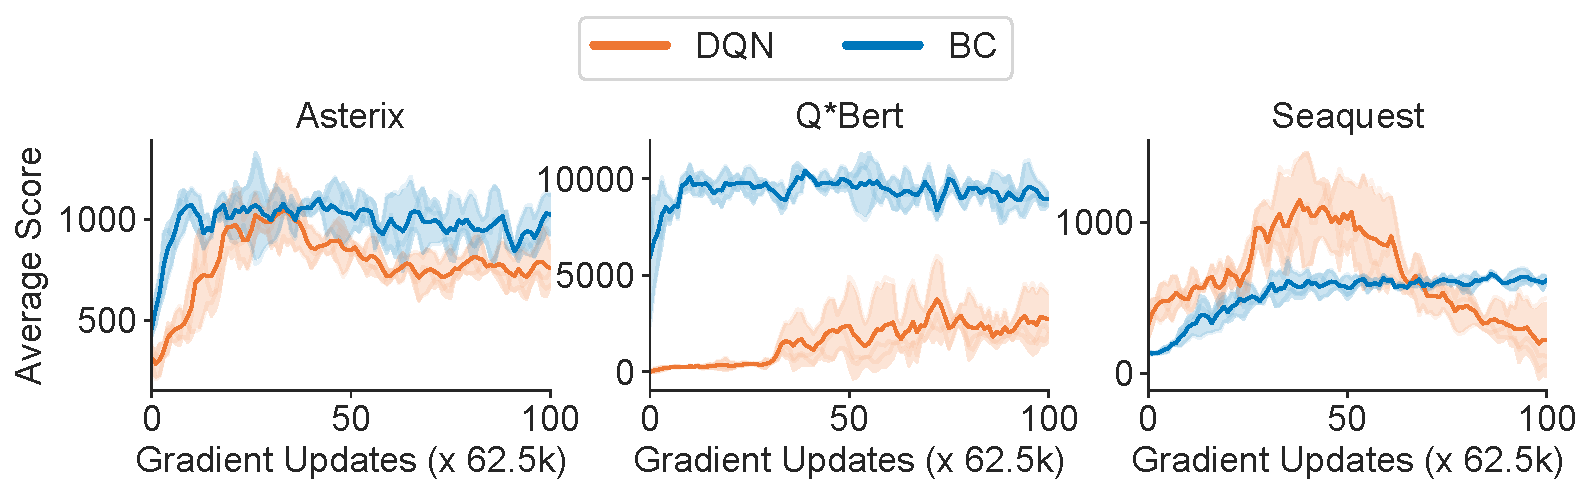
\includegraphics[width=\linewidth]{atari/perf_3_games.pdf}
    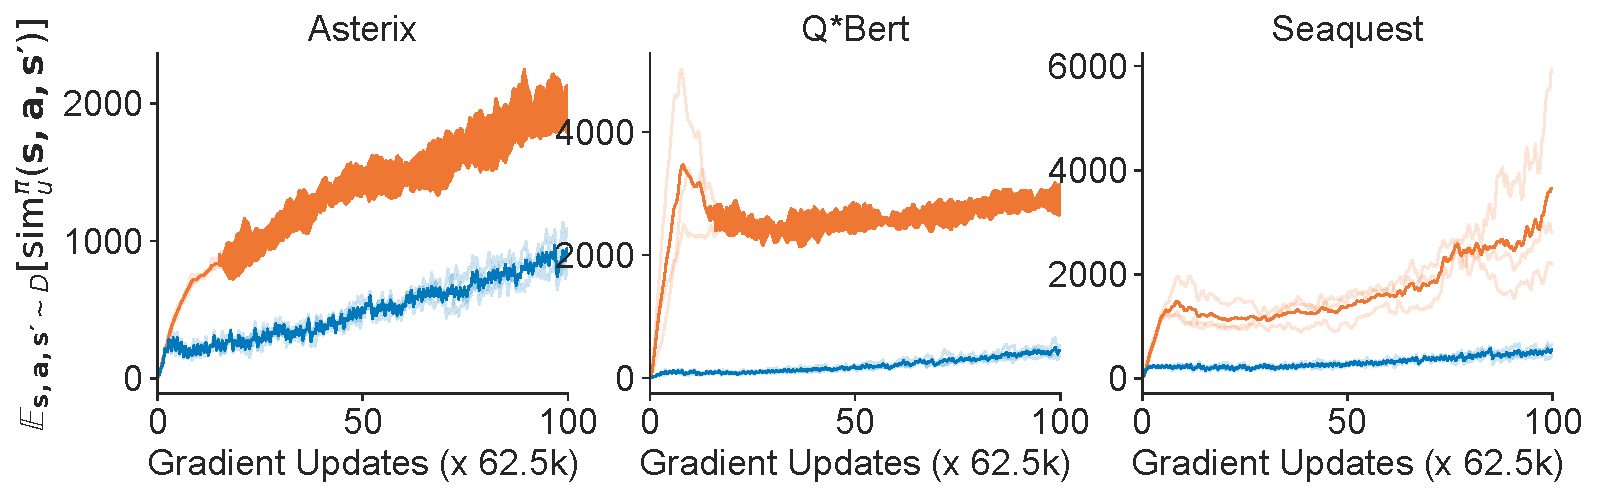
\includegraphics[width=\linewidth]{atari/unnorm_3_games.pdf}
    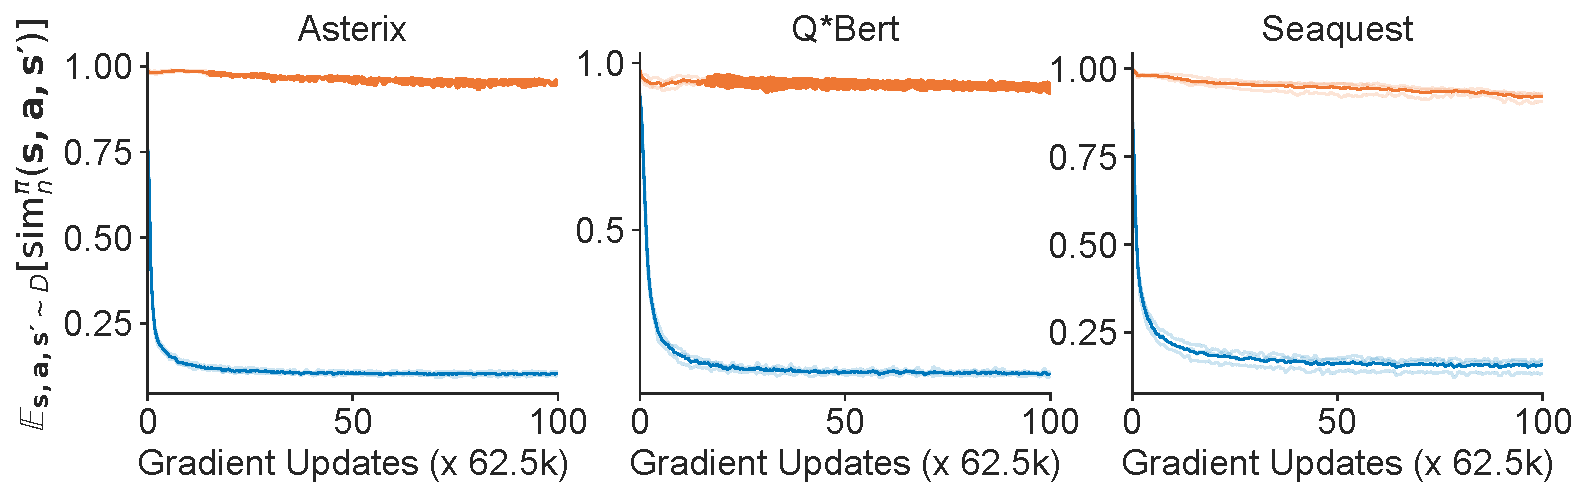
\includegraphics[width=\linewidth]{atari/norm_3_games.pdf}
    \vspace{-0.65cm}
    \caption{\small{Performance of offline DQN and BC on 5\% DQN replay dataset~\citep{agarwal2019optimistic} (top), normalized similarity scores for DQN and BC (bottom). As compared to DQN, $\simnorm$ (cosine similarity) decays significantly faster for BC. 
    \textcolor{red}{Remove the middle row that's not useful. Reduce to 2 games. Also add SARSA}}
    } 
    \label{fig:atari_3_games}
    \vspace{-0.4cm}
\end{wrapfigure}
%% The first para is saying aliasing exists in very simple language
%%SL.5.13: I think before we dive into why it happens, can we just show what the problem is? E.g., show some learning curves where performance peaks and drops, and explain what's going on. Only then talk about *why* it happens
%%AK: sorry for bringing this up again. But I feel like that would make it like iUP basically. I have cited this issue of what happens using a figure later in the paper in the para above as well as citing figure from IUP. We can put a wrapfig in the accompanying text above, but it feels a little copied if we spend the technical section on this. Maybe this is not a good choice. What do you think? 
As noted in~\citep{kumar2021implicit}, one of the most notably visible impacts of representation regularization is the pathological feature aliasing phenomenon that arises with more training. While this aliasing issue has been previously quantified via a collapse in the rank of the feature matrix $\Phi$, this evidence does not shed light on the exact mechanism by which aliasing happens -- even standard supervised learning would exhibit a drop in rank($\Phi$); though not in enormous amounts. % one closing line on how as a result it is less clear how to measure aliasing and connection to bootstrapping empirically.   
%%AK: tried to add a comparison against 

\textcolor{red}{This first part of Section 3.1 will likely be removed in favor of a didactic example} \textit{How can we connect the degree of aliasing to bootstrapping?} Since the difference between bootstrapping and standard supervised learning is primarily that the Q-function at $(\bs, \ba) \in \mathcal{D}$ is trained  with targets generated using Q-values at $(\bs', \ba')$ instead of fixed targets, excessive similarity between $\phi(\bs, \ba)$ and $\phi(\bs', \ba')$ leads to highly coupled Q-values on the two sides of the Bellman update, which can lead to issues such as overestimation and divergence~\citep{durugkar2018td}. Hence, it is informative to measure the similarities in representations $\phi(\bs, \ba)$ and $\phi(\bs', \ba')$. We measure two notions of similarity: \textbf{(1)} we measure the cosine similarity between $\phi(\bs, \ba)$ and $\phi(\bs', \ba')$, and \textbf{(2)} we measure an aggregate    

Observe in  Figure~\ref{fig:atari_3_games} that perhaps surprisingly the similarity between $\phi(\bs, \ba)$ and $\phi(\bs', \ba')$ decreases and saturates at low values with behavior cloning (BC),
%%SL.5.13: This feels like a non-sequitur -- you're comparing representations at two different states, why does it matter that BC is trying to match the behavior policy?
On the other hand, DQN, which is trying to actually improve upon the behavior policy, essentially aliases
%%SL.5.13: There is no evidence of aliasing, just of high dot product (which is not the same)
feature representations at $(\bs, \ba)$ and $(\bs, \ba')$, giving rise to very high similarity values.
%%SL.5.13: Without more context about what's going on, I would say at this point that this is probably due to the OOD actions problem you mentioned before, which DQN does nothing to fix. Additionally, I think it's very likely that many reviewers at this point woudl complain that it's non-sensical to compare BC (which learns policies) with DQN (which learns Q-functions).
This indicates that, compared to supervised learning (e.g., BC), implicit regularization effects in deep Q-learning have a tendency to alias predictions at states and corresponding next states. \textcolor{red}{Would be good to show this with SARSA vs MC: that way we can make a stronger statement like: Note that while both SARSA and MC returns are essentially computing the same quantity and differ only in the nature of implicit regularization induced. This difference makes a huge difference -- in one case, representations at consecutive states are essentially completely aliased, while supervised learning is able to disentangle representations.}
%%SL.5.13: Overall, I think this paragraph is rather problematic. If you want to explain this part, it would be good to really slow it way down and walk the reader through it much more slowly, otherwise so many of the choices in the above paragraph come across as ad hoc, making the conclusions unconvincing.

\fi

\subsection{A Didactic Example}
\label{sec:empirical_analysis}

As noted in~\citep{kumar2021implicit}, one of the most notably visible impacts of representation regularization is the pathological feature aliasing phenomenon that arises with more training. While this aliasing issue has been previously quantified via a collapse in the rank of the feature matrix $\Phi$, this evidence does not shed light on the exact mechanism by which aliasing happens -- even standard supervised learning would exhibit a drop in rank($\Phi$) with more training, and while prior work shows that bootstrapping exacerbates it empirically, it is unclear how exactly this amplification happens. In this section, we describe the intuition behind this mechanism with a didactic example of a 2-action, 1D line MDP~\citep{dong2020expressivity} with a piece-wise linear deterministic dynamics function, $P(\bs'|\bs, \ba) = \mathbb{I}(\bs' = f(\bs, \ba))$ shown in Figure ??. The reward $r(\bs, \ba)$ at any state is the value of the state itself, i.e., $r(\bs, \ba) = \bs$.

The optimal Q-function for this MDP is shown in Figure ??, and 3-layer deep ReLU network Q-functions estimators learned via supervised regression and TD-learning on the identical finite dataset are shown respectively in Figures ?? and ??. While neither supervised regression nor TD learning can learn the complete structure of the optimal Q-function, TD learning fails to represent important high-frequency components of the Q-function (marked in yellow), leaning a ``simple'', smooth Q-function. Since it fails to model the changes in the Q-function well, the resulting policy often chooses the worse action. Quantitatively, the policy extracted from such a TD Q-function is worse than that extracted from the supervised Q-function at more than half the states.  
%%AK: todo: mark in yellow via keynote

%% The next para is saying aliasing is undesirable
\textbf{Why do we observe overly smooth Q-functions in the didactic example when trained with TD learning?}  While excessive aliasing of internal representations in the neural network is expected to generally lead to poor performance, aliasing between $\phi(\bs, \ba)$ and $\phi(\bs', \ba')$ is especially detrimental when learning with Bellman backups. Intuitively, since Bellman backups train features such that the difference of Q-values, $Q(\bs, \ba) - \gamma Q(\bs', \ba')$ matches the reward function, $r(\bs, \ba)$, only on a finite number of state-action tuples seen in the dataset, the features $\phi(\bs, \ba)$ and $\phi(\bs', \ba')$ can learn to only be sufficiently different to predict the reward, thereby achieving low TD error and may be excessively regularized otherwise, thus not capturing long-term structure in the Q-function. Put in other words, there are many possible assignments of weights to a function approximator that could give rise to equally low TD error at the cost of varying degrees of aliasing or regularization.

%%SL.5.13: This feels really hand-wavy. I'm also not sure I agree with this argument -- after all, how would it be any different if there *wasn't* aliasing? Wouldn't you still get a good fit between the difference and reward? This kind of a makes a non-falsifiable statement.
%%AK: this figure is like the example in the MB vs MF paper, but with Bellman backups run on it.

\begin{wrapfigure}{r}{0.5\textwidth}
    \centering
    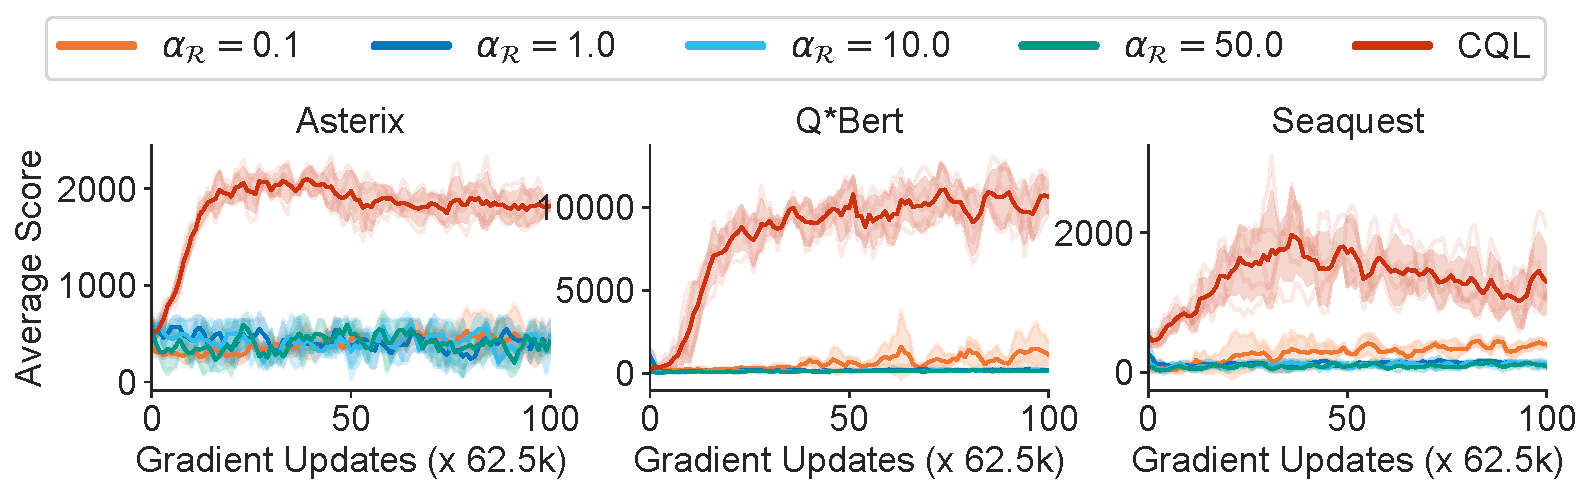
\includegraphics[width=\linewidth]{atari/cql_on_bootstrapping_feat.pdf}
    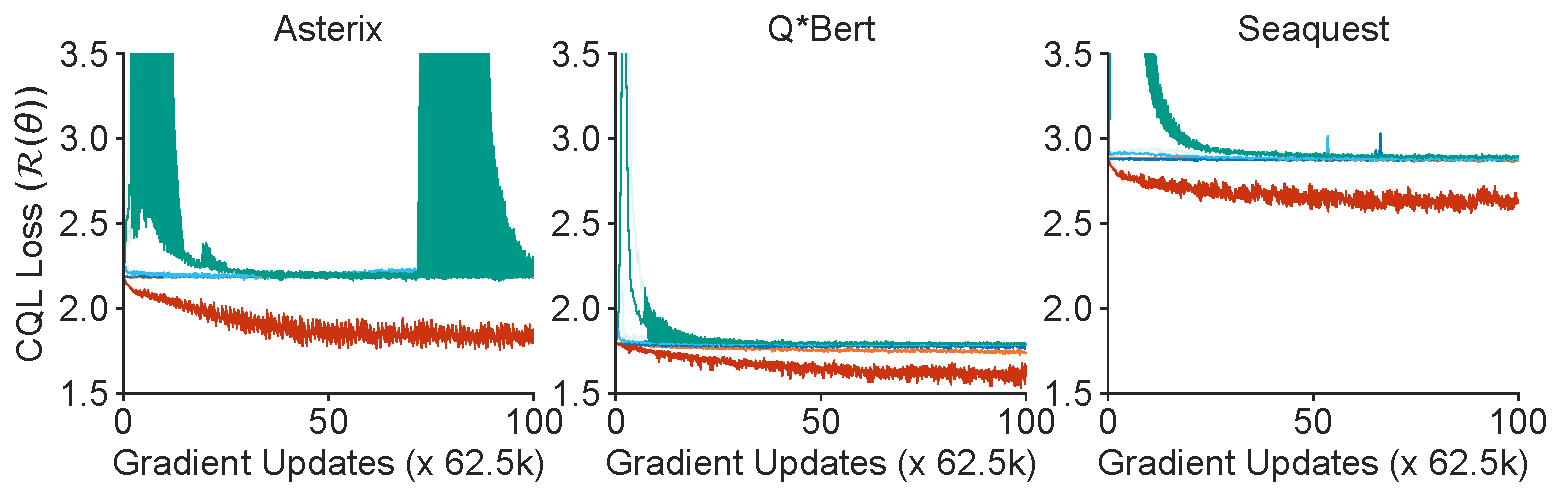
\includegraphics[width=\linewidth]{atari/cql_losses_bootstrapped_feat.pdf}
    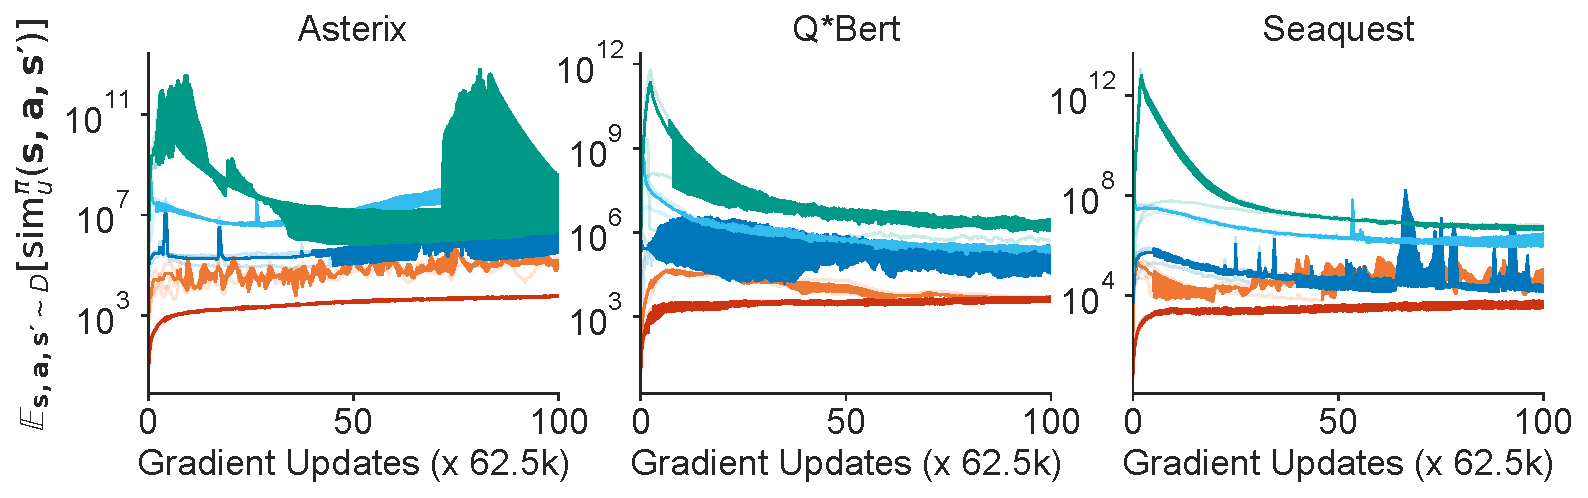
\includegraphics[width=\linewidth]{atari/sim_s_ns_cql_on_bootstrapping_feat.pdf}
    \vspace{-0.65cm}
    \caption{\small{CQL($\phi$), trained using 5\% DQN replay dataset, that learns on features trained solely via bootstrapping where the CQL regularizer $\mathcal{R}(\theta)$ only updates the linear weights of the Q-network. Different values of $\alpha_R$ correspond to different strengths of conservative regularization. We also show standard CQL~(red) for comparison.}} 
    \label{fig:atari_3_games_cql_bootstrap}
    \vspace{-0.6cm}
\end{wrapfigure}
When excessive aliasing is induced by such a mechanism, even modern offline RL methods that are meant to prevent against distributional shift
%%SL.5.13: It's unclear what preventing distributional shift has to do with this
are rendered ineffective. To demonstrate this empirically, we trained a modified version of CQL~\citep{kumar2020conservative}, CQL$(\phi)$, that learns on features $\phi(\bs, \ba)$ solely trained via bootstrapping, and the CQL regularizer is allowed to only update the last linear layer weights. As shown in Figure~\ref{fig:atari_3_games_cql_bootstrap}, no strength of conservative regularization is able to minimize out-of-distribution Q-values resulting in higher values of CQL loss and significantly worse performance as compared to CQL. This indicates that, no matter what, aliased representations can significantly hamper the efficacy of offline RL methods.
%%SL.5.13: This experiment seems weird. You said (and showed before) that features learned with bootstrapping are bad, and it seems like now you are saying if you take those features and retrain, it's still bad, but that's not surprising. I think the subtlety here is that you are also showing that the CQL regularizer is ineffective, but that seems obvious? And it also requires a degree of familiarity with CQL to understand, that the reader might not have. Maybe we can do away with this paragraph?

%%AK: this is the experiment where we initialize the Q-function from a good checkpoint and show it still performs poorly so it is reasoning about the stability aspect.
Finally, to demonstrate the detrimental extent of this implicit regularization on stability of the offline RL algorithm, we perform a controlled experiment where Q-learning is initialized from a ``good'' Q-function that doesn't exhibit aliasing.
%%SL.5.13: where does this come from?
As shown in Figure ??,
%%AK: TODO(AK): add figure!
more learning iterations with modern offline RL algorithms can still drive the algorithm away from this good solution towards more aliased and poor performing solutions. This shows that aliasing caused due to the implicit regularization of training does not just affect the peak performance of an algorithm, but also plays a significant role in destabilizing algorithms when they reach their peak performance.  

\subsection{Theoretical Analysis of Implicit Regularization in Offline Deep Q-Learning}
\label{sec:theory_evidence}
%%SL.5.13: Calling this "implicit regularization" seems premature -- all we showed is that features get larger dot products, which doesn't mean there is some sort of "implicit regularization" going on
In this section, we formalize our empirical observations from Section~\ref{sec:empirical_analysis} and provide a theoretical analysis of the implicit regularization issue. We aim to answer two questions: \textbf{(1)} How do implicit regularization effects in TD learning affect the the aliasing of representations at consecutive states used in the Bellman update? and, \textbf{(2)} How does excessive aliasing affect performance of the algorithm? To answer these questions, we first introduce a simple abstract model of neural network behavior
%%SL.5.13: Rephrase as something like: we first introduce a simple abstract model of neural network training dynamics in value-based RL, and then use this model to analyze the effect of repeated SGD updates on the TD objective. [or something like that]
that allows us to answer these questions.

% abstract model
%% AK: TODO (AK): Also check if we can generalize this to arbitrary continous domains
%%SL.5.13: In its current form, I'm a bit nervous about this version of the theory. I think the SGD implicit regularization version is more convincing and makes fewer arbitrary choices. I do think this version could be made better if we can get rid of the discrete set though. Would be good to get Tengyu's take on it too...
\textbf{Abstract model.} Our abstract model captures feature learning as making a discrete selection among $K$ different feature vector candidates, $\{\Phi_1, \Phi_2, \cdots, \Phi_K\}$, $\Phi_i \in \mathbb{R}^{|\data|\times d}$,
%%SL.5.13: It would be way easier to understand if we could get continuous domains, and then just frame this as an optimization over \Phi (i.e., optimization over \Phi corresponds to selecting the best \Phi \in [some set]), that way we don't have to have this "discrete selection" business and could just say that it's part of the optimization process.
and then training a linear layer $\bw \in \mathbb{R}^{d}$ to obtain the Q-function.
%%SL.5.13: One way you could phrase is this: Our abstract model of the learning process separates the neural network into two parts: a representation $\Phi$ and a weight vector $\bw \in ...$, such that the full model is given by $\Phi(..)^T \bw$ (i.e., $\bw$ corresponds to the last linear layer). The learning process is framed as a \emph{bilevel} optimization problem, where the weights $\bw$ are chosen subject to a constraint that the learning process chooses the optimal features $\Phi \in [set]$ for $\bw$ (or something like that)
To mimic the overparameterized nature of neural networks, we assume that we operate in the overparameterized regime with $n < d$.
%%SL.5.13: This is kind of weird -- usually the last layer features are not that high dimensional, but the model parameters are. Are you sure we shouldn't look for some way to "NTK-ify" this? Perhaps a better way to frame this is that we are in the NTK regime where the choice of Phi corresponds to the choice of NTK (i.e., it's not fixed, as is more common in this analysis), while bw corresponds to the neural net parameters? That would justify the overparameterized regime and make this less weird.
Assume that the initial value of the weight vector $\bw^{(0)} = 0$. We then write out the minimum-norm optimization problem shown below in Equation~\ref{eqn:min_norm} that attains the same solution as the optimal solution found by minimizing training TD error in this model, and characterize the properties of features $\Phi_K^*$ that are selected to obtain the minimum-norm solution. \textcolor{red}{more assumptions?}     
%%SL.5.13: It won't be clear to some people what min-norm has to do with neural net training, can you cite something to justify this?
\begin{align}
    \min_{\bw, \boldm_i \in \{0^d, 1^d \}}~~& ||\bw||_2^2 \nonumber\\
    \text{s.t.}~~&~ \bar{\Phi}^\top \bar{\Phi} \bw = \bar{\Phi}^\top R + \gamma \bar{\Phi}^\top P^\pi \bar{\Phi} \bw, ~~ \bar{\Phi} = \left[\Phi_1, \cdots, \Phi_k\right] \otimes [\boldm_1, \cdots, \boldm_K]
\label{eqn:min_norm}
\end{align}
%%SL.5.13: ouch, this \bm_i is... difficult to parse
Our first result characterizes the feature representation $\bar{\Phi}$ -- equal to one of $\Phi_i$ selected based on the learned masks $\bm_i$ -- that satisfies the Bellman consistency condition but also minimize the implicit regularizer, $||\bw||_2^2$,
%%SL.5.13: where does this implicit regularizer come from?
and use this to depict the existence of this phenomenon.

\begin{theorem}
\label{thm:aliasing_exists}
Let the singular value decomposition of $\Phi_i$ be given as $\Phi_i = \bU_i \Sigma_i \bV_i^\top$ and $\bw^{(*)}, \boldm^{(*)}$ minimize the objective in Equation~\ref{eqn:min_norm}. Assume that the reward vector lies in the column space of $\Phi_i$, $\forall i \in [K]$, i.e., $\exists~ y_i, R = \Phi_i y_i $.  Then, $\bar{\Phi}$ is such that:
\begin{equation*}
    \bar{\Phi} := \arg \min_{i}~ \big|\big| \Sigma_i^{-1} \left( \bU_i^T (I - \gamma P^\pi) \bU_i \right)^{-1} \Sigma_i y_i\big|\big|_2^2.
\end{equation*}
Thus, the resulting $\bar{\Phi}$ satisfies: $\mathrm{srank}\left(\bar{\Phi}^\top (\bar{\Phi} - \gamma P^\pi \bar{\Phi}) \right) \leq \mathrm{srank}\left(\Phi_i^\top (\Phi_i - \gamma P^\pi \Phi_i) \right)~ \forall i$, which quantifies the existence of aliasing between representations at consecutive states in TD-learning.
\end{theorem}
%%SL.5.13: It's not clear what this last sentence means ("which quantifies the existence of aliasing between representations at consecutive states in TD-learning") -- can we state the implication of this theorem more precisely. As written, it's also not clear what this theorem has to do with SGD (I guess it's the min-norm part?).

%%SL.5.13: It might also help with clarity to explain why this problem *doesn't* happen in the supervised learning case

A proof of Theorem~\ref{thm:aliasing_exists} can be found in the Appendix ??. The main consequence of this result is a characterization of the learned features at optimal TD solutions in our abstract model in terms of the effective rank~\citep{kumar2021implicit} of the matrix $\bM(\Phi) := \Phi^\top (\Phi - \gamma P^\pi \Phi)$. A low rank of $\bM(\Phi)$ for a given rank of $\Phi$ intuitively indicates that the basis of the difference in features at consecutive states, $\Phi - \gamma P^\pi \Phi$, heavily lies
%%SL.5.13: try to avoid hand-wavy language ("heavily lies") and state what you mean more precisely
in the null space of the feature matrix $\Phi$, as a result of which the weight vector $\bw$ will be updated only in a few directions allowed by both $\Phi$ and $\Phi-\gamma P^\pi \Phi$.indicating that only a partial set of features will actually be used for learning.
%%SL.5.13: something is malformed above ("indicating that")
To empirically verify the existence of such an aliasing phenomenon, following the procedure outlined in \citep{kumar2021implicit}, we measure the effective rank of $\bM(\Phi)$ and observe in Figure ?? that this matrix indeed has extremely low rank when training with TD backups, as compared to supervised regression.
%% AK: this supervised regression is BC. Should we also do this for something else?

%%AK: maybe write the stuff below as a theorem?
Another interesting consequence of Theorem~\ref{thm:aliasing_exists} is the effect of the ``simplicity'' of the reward function on feature aliasing. We define simplicity by the number of non-zero components in the vector $y_i$.
%%SL.5.13: maybe we should avoid ad hoc definitions like this, and try to just state this more plainly and directly?
As an extreme case, note that if the vector $y_i$ has all zeros, except a single 1 entry, the optimal $\bar{\Phi}$ is expected to induce $\bM(\Phi)$ with a much lower rank compared to when a significantly more number of values of $y_i$ are non-zero (as shown in Appendix ??).
%%SL.5.13: this seems imprecise ("much lower")
This means that when the reward function $R$ actually non-trivially combines the singular vectors of $\Phi$ -- which we refer to as a ``complex'' reward function -- the effective aliasing
%%SL.5.13: I think if you're going to use the term "aliasing" like this, it needs to be formally defined. Aliasing means that two things are indistinguishable (not similar, but indistinguishable). The word is being used in a different way here.
is little less than when it does not. We indeed observe this behavior in practice, as shown in Figure ?? in Section~\ref{sec:empirical_analysis}, and our abstract model sheds light on how this implicit regularization effect in TD-learning is exacerbated in scenarios where reward functions can be expressed using very few components of the feature matrix $\Phi$.
%%SL.5.13: how do you know if it can be expressed using very few components?
%%SL.5.13: I think I understand what you are trying to say in the above paragraph, but we need to find a cleaner and more concise way of saying it. Maybe what we can say is something like -- consider the projection of the reward function onto the column-space [?] of Phi, with coefficients ??. If these coefficients are sparse, we would expect [??] (try to be precise!)...

To conclude our analysis for question \textbf{(1)}, we finally note that an analogous result in supervised learning would indicate no existence of any implicit bias that preferentially aliases feature representations at consecutive states. While prior work \citep{kumar2021implicit} has also generally shown the compounding effect of implicit regularization towards low-rank $\Phi$ in TD-learning, our analysis explicitly identifies the structure of aliasing induced by this implicit regularization: the rank of the matrix $\bM(\phi)$ drops, leading to aliasing at consecutive states.
%%SL.5.13: It's good to have a paragraph like the one above, but it addresses two things simultaneously, and doesn't do either very well: the supervised learning bit seems to have no punchline (so... is this a contradiction? if not, why not?); the bit about IUP doesn't clearly state how what you are showing is different from IUP.

%%SL.5.13: Given how long-winded the above is, maybe consider a subsection heading for (2) or something (or at least paragraph heading)
Next, we answer question \textbf{(2)} regarding the detrimental impacts of aliasing. 
\textcolor{red}{Need to finish this bit -- there are some options we can go: (1) We can show that there exist MDPs with simple reward functions and complex Q-functions, where such an implicit regularizer will cause the MDP to learn overly smooth Q-functions. (2) We can show that even when initialized close to a good solution, this implicit regularizer will drive the model towards picking features that are the most aliased, in which case we do not even stabilize near a good solution even if we reach it. (3) We could show that distributional shift correction on top of aliased features will not work, similar to what we had before the ICML deadline. Which of these option(s) should we prefer?}

\fi






















%%%%%%%%%%%%%%%%%%%%%%%%%%%%%%%%%%%%%%%%%%%%%%%%%%%%%%%%%%%%%%%%%%%%%%%%%%%%%%%%
%%%%%%%%%%%%%%%% old stuff below %%%%%%%%%%%%%%%%%%

\iffalse
\section{\AliasingProblemName\ in Offline RL}
\label{sec:problem}
%%SL.2.3: Kind of a nitpick, but "Bootstrapping Aliasing" kind of makes it sound like we are bootstrapping the aliasing (rather than that we have aliasing that stems from bootstrapping). But why do you want "bootstrapping" in the name? It doesn't really have anything to do with bootstrapping, at least not moreso than anything else that relates to RL. It's kind of more like Policy Aliasing (or something like that...)

Empirically, we find that the combination of neural network function approximators, bootstrapping, and minimizing TD error 
% with gradient descent 
leads to aliasing
%%SL.2.3: Aliasing between what and what?
of the state-action pairs appearing in a Bellman update. Minimizing TD error against bootstrapped targets uses a tuple $(\bs, \ba, \bs')$ from the dataset, draws an additional action sample from $\pi(\cdot | \bs')$, which may not be observed in the dataset, and evaluates $Q_\theta(\bs, \ba)$ and $Q_\theta(\bs', \ba')$. We find that the features $\phi(\bs, \ba)$ and features $\phi(\bs', \ba')$ become aliased over the course of learning,
%In this section, we will see how offline training of Q-functions by minimizing TD error against a bootstrapped target value estimate \emph{aliases} feature representations on actions drawn from the dataset $\phi(\bs, \ba)$ and the feature representations on actions from the learned policy that will be used for bootstrapping, but are not observed in the dataset, which we denote as $\phi(\bs', \ba')$. Since features $\phi(\bs', \ba')$ directly influence the features at dataset state-action tuples $\phi(\bs, \ba)$ via the bootstrapping update, a similarity between features at these specific state-action tuples is likely to affect optimization dynamics of the algorithm as we will more formally discuss in Proposition~\ref{thm:separability}.  
%%AK.2.3: I don't know how to motivate this, I wrote something up but this isnt convincing 
%%SL.2.1: which we denote as
and we refer to this phenomenon as \emph{\aliasingproblemname}.
%%SL.2.3: As stated, this sounds a little bit silly, because \bs and \bs' are very similar, so of course they are likely to be aliased! I think it would help to explain the *policy* aliasing part first, and then explain that a particularly prominent instance of this has to do with \ba and \ba' (but FWIW, I still think we are making too big of a deal out of the fact that these are sequential actions, and things would be much clearer and less likely to be misunderstood if we did not do this, and instead focused on policy aliasing and brought in the s/a/s'/a' stuff as late as possible)
To measure this aliasing, we use the normalized and unnormalized dot product similarities %To begin, we formally define two metrics to quantify \aliasingproblemname, and then demonstrate the existence of this issue in offline Q-learning methods.
\begin{align*}
    \simnorm(\bs, \ba, \bs'; \phi) &:= \frac{|\phi(\bs, \ba)^T \E_{\pi(\ba'|\bs')}[\phi(\bs', \ba')]|}{||\phi(\bs, \ba)||_2 ||\E_{\pi(\ba'|\bs')}[\phi(\bs', \ba')]||_2},\\
    \simunnorm(\bs, \ba, \bs'; \phi) &:= |\phi(\bs, \ba)^T \E_{\pi(\ba'|\bs')}[\phi(\bs', \ba')]|.
\end{align*}
%\begin{definition}
%\emph{\Aliasingproblemname} is said to happen when features $\phi(\bs, \ba)$ on $(\bs, \ba, \bs') \in \data$ and the expected feature vector on actions drawn from the learned policy $\pi(\cdot |\bs')$ at the next state $\bs'$, $\E_{\ba' \sim \pi(\cdot|s')}[\phi(\bs', \ba')]$, exhibit a high normalized or unnormalized dot product similarity on an average over the dataset $\mathcal{D}$. The normalized ($\simnorm$) and unnormalized ($\simunnorm$) similarities are given by:
%%%SL.2.1: It's unclear why you are using a/a' on successive timesteps. Since this is a definition, it might come across as weirdly arbitrary. Beyond this, there is the question of whether this is referring to this quantity in expectation over s, on average, etc.
%%%AK.2.3: I don't know how best to do that. I want to write this section as policy indistinguishability, where we measure (s, a), (s, a') similarity, but that doesn't seem to be the case we can make in time
%\begin{align*}
%    \simnorm(\bs, \ba, \bs'; \phi) &:= \frac{|\phi(\bs, \ba)^T \E_{\pi}[\phi(\bs', \cdot)]|}{||\phi(\bs, \ba)||_2 ||\E_{\pi}[\phi(\bs', \cdot)]||_2},\\
%    \simunnorm(\bs, \ba, \bs'; \phi) &:= |\phi(\bs, \ba)^T \E_{\pi}[\phi(\bs', \cdot)]|.
%\end{align*}
%\end{definition}
We omit $\phi$ when it is clear from context. %A high $\simnorm$ indicates state-action tuples $(\bs, \ba) \sim \mathcal{D}$ and the next state-action tuple, $(\bs', \ba')$ where $\ba' \sim \pi(\cdot|\bs')$ are directionally aligned,
%%SL.2.1: Above sentence appears to (intentionally?) omit saying what the state is, just saying the action. Especially combined with the s/s'/a/s' confusion in the previous definition, this might be not so great
%%AK.2.3: added this 
%whereas the feature magnitude captured in $\simunnorm$ indicates the extent to which directional similarity affects optimization~(Section~\ref{sec:analysis}). As a result, by tracking average similarities over the dataset, $\E_{\bs,\ba, \bs' \sim \data}[\simnorm(\bs, \ba, \bs')]$ and $\E_{\bs, \ba, \bs' \sim \data}[\simunnorm(\bs, \ba, \bs')]$,
%%SL.2.1: This average thing seems a bit hacky.
%%AK.2.3: introduced the average bit in the definition above
%we can verify the existence of \aliasingproblemname.
Intuitively, this could be problematic in the offline RL setting where carefully controlling generalization is critical to performance~\citep{levine2020offline}
%%SL.2.3: I don't really understand what claim this reference is supposed to be supporting
because it couples the $Q$ values of $(\bs, \ba)$ and a potentially out-of-distribution tuple $(\bs', \ba')$.
%%SL.2.3: should clarify that it's the action that's OOD, not the state (lest someone misunderstand)
% For example, assume that the features $\phi(\bs, \ba) \in \mathbb{R}^d$ are positive (as is the case with ReLU activations) and unit norm, then $\simnorm(\bs, \ba, \bs') \geq 1 - \varepsilon$ immediately implies that $(Q_\bw(\bs, \ba) - \E_{\pi(\ba'|\bs')}\left[Q_\bw(\bs', \ba')\right])^2 \leq 2\varepsilon||\bw||_2^2$.
%%SL.2.3: This early in the paper, the significance of this inequality is not clear (indeed, it's not clear to me even, and I've read the whole paper many times!)
In the next subsections, we present empirical evidence demonstrating that bootstrapping induces \aliasingproblemname\ and then discuss its consequences, before using these insights to develop \methodname\ in Section~\ref{sec:method}.  

%%SL.2.1: Overall, I'm concerned that there are a number of details in this section that make what would otherwise be a fairly clean exposition kind of confusing. Namely, the fact that there are two similarity measures, and the s/a/s'/a' thing. Perhaps in the interest of clarity we can simplify this? Not sure how well that would still fit with what follows later, but it seems like something we can do better. Beyond this, it's not clear why high "indistinguishability" is actually "indistinguishable" -- if the features are perfectly aligned, of course they are indistinguishable, but I do think that many readers will have the same criticism here that I had -- if the similarity is high but not perfect, then the features really are distinguishable, just the differences are smaller. We probably don't have room to do this concept justice in this section, but at least providing a little bit of intuition and/or a forward reference about it here would I think help.
%%AK.2.3: I edited this, does it seem better?


%%AK.1.31: discuss IUP in the related work section, TODO!
\subsection{High \AliasingProblemName\ During Training}
\label{sec:bootstrapping_evidence}
To study how $\simunnorm$ and $\simnorm$ evolve over the course of training with offline RL, we measure both quantities during training on three Atari games in \Figref{fig:atari_3_games}.
On each game, we run standard DQN~\citep{Mnih2015} on an offline dataset that consists of partially subsampled experience from an online Atari agent~\citep{agarwal2019optimistic}. For comparison, we visualize the corresponding metrics for supervised learning behavioral cloning and offline SARSA~\citep{rummery1994line} that uses the actions from the dataset at the next state for bootstrapping updates. First, note that both $\simnorm$ and $\simunnorm$ are an order of magnitude higher for DQN, as compared to supervised BC, \emph{despite the fact that BC is trying to directly match the behavior policy}, whereas DQN is trying to improve upon the behavior policy and intuitively representing the behavior policy from the learned policy is crucial for improvement. Furthermore, since there are no out-of-distribution actions used in SARSA, the \aliasingproblemname\ is more severe in DQN compared to SARSA.
%%SL.2.1: \emph{despite the fact that BC is directly trying to match the behavior policy}, while DQN is trying to improve on it
%%RA.2.2: I didn't understand why "despite" the fact -- do we expect BC's similarities to be higher?
%%AK.2.3: added the intuition
As compared to DQN, $\simunnorm(\bs, \ba, \bs')$ increases much slower for BC and SARSA while $\simunnorm(\bs, \ba, \bs')$ decays significantly faster for BC and SARSA.
%Note that these values also generally exhibit an increasing trend with DQN, but a relatively stable trend over more training for BC.
Furthermore, we observe a similar trend of large $\simunnorm$ and $\simnorm$~(\Figref{fig:atari_3_cosine}) during training for offline RL algorithms that address distributional shift, such as CQL~\citep{kumar2020conservative} and REM~\citep{agarwal2019optimistic}. Based on this evidence, we ask: 
%RA.2.3: Does the \aliasingproblemname\ issue happen consistently, or is this merely an accident? 
what are the consequences of \aliasingproblemname\ on algorithm performance? 
%RA.2.3: We will show in Section~\ref{sec:analysis} that bootstrapping combined with gradient descent indeed amplifies these similarity metrics, particularly $\simunnorm$.

%%AK.1.31: reword/remove the para below, if we actually arent able to show something from the min-norm problem.

% Can we improve performance by addressing this issue? 
%We investigate this question in the next section, and then propose \methodname\ that mitigates \aliasingproblemname\ and leads to more effective offline RL in practice.

%%SL.2.3: When we shuffles things around in the paper, I think we might have removed something from this section, because as written, it doesn't actually motivate anything significant: it just says this mysterious quantity we defined (and that we decided to call "aliasing") is higher for some methods than others. But right now, as far as I could tell, this section doesn't actually say anything about how this is *bad*. That seems like a problem, because the reader will probably think that we're just saying random stuff in this section, and might simply stop reading.



\subsection{Consequences of High \AliasingProblemName}
\label{sec:consequences_of_feature_sim}
%In this section, %we discuss the consequence of high feature similarity on the performance of offline RL algorithms. 
%we analyze the behavior of offline Q-learning when \aliasingproblemname ~is high.
%%%SL.2.1: I don't get this last part -- why does it correct for it "when $\simnorm$ and $\simunnorm$ are high"?
%%%RA.2.1: The previous sentence was confusing, what we mean is that the analysis is done when feature similarities are high.
%Our intuition is that with high similarities, the Q-function is unable to distinguish between dataset and out-of-distribution actions or it needs to learn high magnitude values in order to meaningfully distinguish between them, in which case it can no more a valid Q-function for the MDP (that takes on possible values for expected return in the MDP). 
%As a theoretical abstraction, we show in Theorem~\ref{thm:separability} that for a given offline dataset $\data$, %of size $|\data| = n$, 
%the probability of a large margin between the Q-values at  $(s, a) \sim \data$ and $(s, a) \sim \data, \pi$
%%%SL.2.1: As before, it seems like here there is a bit of cleverness in omitting which state this depends on -- but that detail is important. Of course actions at different states will have different representations...
%%%AK.2.3: addressed
%computed via a linear transformation on the features decreases with normalized similarities $\simnorm$.
%This implies that a valid Q-function  learned by any offline RL algorithm, even when it corrects for distributional shift, will not be able to push down the values of out-of-distribution actions by a large margin.
%%%SL.2.1: I'm not really sold on this statement. Is there a reason to believe that a numerically smaller margin implies that it is harder to distinguish things? Just scaling down the features by a constant factor as I had mentioned before would also have this property, but of course we wouldn't argue that this makes it any harder...
%%%AK.2.1: I edited this above to make it clear we are talking about the Q-function and not the margins of the representations independently. In a setting when I can drive the linear weights to infinity, the margin will be high, but here we can't as we will not have a valid Q-function at that point, and we will have ignored the reward maximization part. 
%% This induces brittleness~\citep{bellemare2016increasing}
%% %%SL.2.1: brittleness?
%% in the learning procedure, and stochasticity and randomness in optimization can lead to issues such as excessive overestimation~\citep{kumar2020conservative} and policy unlearning~\citep{levine2020offline}.
%%%SL.2.1: I would make the second clause (, and...) be a separate sentence, and explain it more explicitly -- are you trying to say that when \simnorm is high, stochasticity in optimization can lead to issues? or something else? it's just a pretty complex phrase to parse
%%%AK.2.3: removed this
%% We first state the result and then empirically validate it.
%\begin{proposition}
%\label{thm:separability}
%Assume that features $\phi(\bs, \ba) \in \mathbb{R}^d$ of the Q-function are uniform random vectors satisfying $\forall~ \bs, \ba, \bs' \in \data,~ ||\phi(\bs, \ba)||_2 = 1,\ \mathrm{and}\ \simunnorm(\bs, \ba, \bs') = \simnorm(\bs, \ba, \bs') \geq \sqrt{1 - \varepsilon^2}$. Let $f_{\bw_c}(\bs, \ba) = \bw_c^T \phi(\bs, \ba)$ be any linear classifier that separates $\data_{\mathrm{in}} = \{(\bs, \ba)\}$ and $\data_{\mathrm{OOD}} = \{(\bs', \ba')\}$, where $\ba' \sim \pi(\cdot|\bs')$. Let $\zeta$ denote the margin obtained by $f_{\bw_c}$ in classifying $\data_{\mathrm{in}}, \data_{\mathrm{OOD}}$, and  assume that classifier weights are bounded, $||\bw_c||_2 \leq \tau$.
%Then, 
%\begin{equation*}
%    \text{Pr} \left(\zeta \geq \alpha \right) \leq \left[ 1 - \left( C_1 \frac{\alpha^2}{\varepsilon^2}\right)^{\frac{d-1}{2}} \right]^{|\mathcal{D}|},
%\end{equation*}
%for some universal constant $C_1 > 0$ that depends on $\tau$.  
%\end{proposition}
%%%SL.2.1: What is the logic for why a small margin makes things bad? We can get a small margin just by making the features small (e.g., dividing them by 1000000), but this clearly wouldn't make the learning problem harder. More generally, I don't think we've really provided the setup that the reader needs to understand why separation between OOD and dataset actions is actually important. Maybe it's more important to establish that?
%%%AK.2.1: I edited this above to make it clear we are talking about the Q-function and not the margins of the representations independently. In a setting when I can drive the linear weights to infinity, the margin will be high, but here we can't as we will not have a valid Q-function at that point, and we will have ignored the reward maximization part. 
%Proposition~\ref{thm:separability} shows that when features are highly similar, \ie small $\varepsilon$, obtaining a Q-function that guarantees a large margin is exponentially smaller than when $\varepsilon$ is large. The proof for Proposition~\ref{thm:separability} can be found in Appendix ??. 
%%%SL.2.1: Why does it show that? I guess your intuition is that if in-distribution and OOD actions are close together, this is hard, but this is not at all obvious
%%AK.2.3: TODO (aviral): put a probability of divergence or something like that

To explore the consequences of \aliasingproblemname, we show that recent methods developed to mitigate the impact of \emph{distributional shift}, such as CQL~\citep{kumar2020conservative}, are ineffective when using features with high \aliasingproblemname. In particular, we evaluate a modified version of CQL, CQL($\phi$), that learns on features $\phi(\bs, \ba)$ trained solely via bootstrapping,
%%SL.2.3: Can you just show basic results first before modifying the method? and can you show things for methods other than cql? eg that regular DQN has high aliasing?
where the CQL regularizer only updates the last linear weight layer of the Q-network~(\Figref{fig:atari_3_games_cql_bootstrap}). As shown in \Figref{fig:atari_3_games_cql_bootstrap}, no strength of the conservative regularization is able to minimize out-of-distribution Q-values resulting in higher values of the CQL loss, and both notions of feature similarity rise to large values during training. Finally, the performance of CQL($\phi$) is significantly worse compared to standard CQL. This provides evidence that \aliasingproblemname negatively impacts performance and suggests that reducing \aliasingproblemname may improve performance.
%%SL.2.3: I think we need more than preliminary evidence, but if more convincing evidence is later, then you can forward reference it
%RA.2.3: while standard CQL on this data can attain a normalized return of 1.0 (gridworld) and ?? (Atari), running CQL on these features attains only 0.6 and ?? respectively.
%%AK.1.31: will there be an issue that why did you have to cripple an algorithm to get this behavior, and why can't this happen by default?

To formalize the intuition from the experiment above, we formally show that with high similarities, the Q-function is either unable to distinguish between dataset and out-of-distribution actions at a given state or it needs to learn high magnitude values in order to meaningfully distinguish between them, in which case it no longer is a valid Q-function estimator for the MDP and suffers from overestimation or underestimation. 
As a theoretical abstraction, we show in Proposition~\ref{thm:separability} that for a given offline dataset $\data$, %of size $|\data| = n$, 
the probability of a large margin between the values at  $(\bs, \ba) \sim \data$ and $(\bs, \ba) \sim \data, \pi$
computed via \emph{any} linear transformation on the features decreases with increases normalized similarities $\simnorm$. Then, the only way available to increase the margins of spearation between values unseen and seen actions is to then scale up either the features magnitudes oe the magnitude of the linear weight vector transforming these features into the -function, both of which lead to overestimation, as is evident in Figure ??. 
%% This induces brittleness~\citep{bellemare2016increasing}
%% %%SL.2.1: brittleness?
%% in the learning procedure, and stochasticity and randomness in optimization can lead to issues such as excessive overestimation~\citep{kumar2020conservative} and policy unlearning~\citep{levine2020offline}.
%%%SL.2.1: I would make the second clause (, and...) be a separate sentence, and explain it more explicitly -- are you trying to say that when \simnorm is high, stochasticity in optimization can lead to issues? or something else? it's just a pretty complex phrase to parse
%%%AK.2.3: removed this
%% We first state the result and then empirically validate it.
\begin{proposition}
\label{thm:separability}
Assume that features $\phi(\bs, \ba) \in \mathbb{R}^d$ of the Q-function are uniform random vectors satisfying $\forall~ \bs, \ba, \bs' \in \data,~ ||\phi(\bs, \ba)||_2 = 1,\ \mathrm{and}\ \simunnorm(\bs, \ba, \bs') = \simnorm(\bs, \ba, \bs') \geq \sqrt{1 - \varepsilon^2}$. Let $f_{\bw_c}(\bs, \ba) = \bw_c^T \phi(\bs, \ba)$ be any linear classifier that separates $\data_{\mathrm{in}} = \{(\bs, \ba)\}$ and $\data_{\mathrm{OOD}} = \{(\bs', \ba')\}$, where $\ba' \sim \pi(\cdot|\bs')$. Let $\zeta$ denote the margin obtained by $f_{\bw_c}$ in classifying $\data_{\mathrm{in}}, \data_{\mathrm{OOD}}$, and  assume that classifier weights are bounded, $||\bw_c||_2 \leq \tau$.
Then, 
\begin{equation*}
    \text{Pr} \left(\zeta \geq \alpha \right) \leq \left[ 1 - \left( C_1 \frac{\alpha^2}{\varepsilon^2}\right)^{\frac{d-1}{2}} \right]^{|\mathcal{D}|},
\end{equation*}
for some universal constant $C_1 > 0$ that depends on $\tau$.  
\end{proposition}

Next, we introduce our approach to fix this \aliasingproblemname\ and demonstrate that reducing \aliasingproblemname leads to significant gains in multiple offline Q-learning methods. %We first present the practical method and then analyze it theoretically. We will then analyze \emph{why} bootstrapping with deep neural networks amplifies the increase in the values of $\simnorm$ and $\simunnorm$.

%%AK.2.3: the stuff below is going to form its new section
\begin{remark}[Connection to offline RL lower-bounds]
Recently, \citet{zanette2020exponential} constructed an OPE problem with linear function approximation that requires exponentially-sized $|\data|$ to meaningfully estimate the value of certain policies. The key idea behind their construction is that the feature vectors $\phi(\bs, \ba)$ and $\phi(\bs', \ba')$ appearing in a Bellman constraint are such that they align with each other and Bellman residual minimization then prevents learning the structure of the reward function crucial for policy evaluation since feature aliasing causes Bellman constraints to form an under-determined system. Our result in Theorem~\ref{thm:bootstrapping} shows that this does not just happen in specific hand-crafted ``worst-case'' MDPs, but is also likely to happen under scenarios~\ref{assumption:magnitude} and \ref{assumption:ood} in several ``average-case'' MDPs when deep neural network value function approximators are used.
\end{remark}
%%SL.1.26: I think making this a "Remark" like this is excessive, maybe this would be easier to explain in paragraph form. It's an important thing to note, and perhaps the relationship to Zanette '20 ought to be brought up earlier, because it in some sense could make the reader more comfortable with our statements about feature collinearity makes RL hard, which otherwise might come across as too vague and informal (simply being *close* does not necessarily make features indistinguishable)

%%SL.2.1: Overall, my sense is that this subsection is not very convincing. I think it's very very heavily dependent on CQL, and it's really trying to say something specific about CQL rather than more general about offline RL. I'm also pretty skeptical that the theorem actually indicates that features with high similarity make learning harder -- nothing about the theorem currently appears to indicate this.

%%%%%%%%%%%%OLD COMMENTS%%%%%%%%%%%

%%SL.1.26: Is the word "aliasing" just used to mean "collinear"? I'm just worried that we are being very loose and vague with terminology...

%%SL.1.26: My suggestion would be to make all the "experiment details" self-contained in an empirical section (e.g., 3.1), so that the reader doesn't mistakenly think that this section is primarily about experiments

%%%AK.1.24: Outline of this section
%%%%PART 1: Problem exists
%% -- Define feature aliasing, show how we can measure it.
%% -- Put out gridworld aliasing plots and show that FQI does suffer from aliasing issues (maybe a film strp of how it evolved would be better), also define an aggregate metric to compare (e.g. entropy of cosine^2 histogram?)
%% -- Put out the same plot for supervised learning, and show a side-by-side comparison that bootstrapping is very different
%% -- Discuss how CQL (and something like BRAC-v) also suffers from this issue and demonstrate plots.

%%% PART 2: Problem Causes Issues
%% -- maybe reuse same figures from before, but show that indeed the issue causes poor performance (especially performance that goes up and drops)
%% -- show some 1 or 2 atari and d4rl plots (and point to appendix)
%% -- theorem 1: when operating in the effective "aligned" regime, it is exponentially harder to fit a meaningful Q-function that both satisfies the conservative constraints and Bellman constraints: and depending upon $\alpha$ and init, divergence is bound to occur either ways -- conservatism or overestimation. Show examples of them (or list some sufficient conditions)

%%% PART 3: Theory behind why the problem exists
%% -- theorem 2: min norm problem for 2 layer relu networks have the affinity of either: 1. overestimation 2. bootstrap off of bad/unseen inputs -- either of them will lead to this issue (i.e. this happens when there is a bad OOD (next state, policy action) tuple used for bootstrapping or even when the Q-values are overestimated)
%% -- remark: bring in the zanette et al 2020 paper, and argue that their lower bound holds due to precisely such featues, and hence even problems which are solvable also suffer from some inabilities to learn due to this aliasing effect.

%%AK.1.24: Any major changes we need to do to the outline?

% \begin{definition}
% \emph{Feature aliasing} refers to increasing value of similarity of features $\phi(\bs, \cdot)$ on state-action pairs present and absent in $\data$ as training progresses. Formally, $\forall~ (\bs, \ba, \bs') \in \mathcal{D}$, the following quantity increases over the course of training training:
% %%AK.1.24: forall s, a might too strict: check on gridworlds, since it seems like this happens on D4RL, but if not on gridworld, change to expectation
% %%SL.1.26: Well, whatever definition you pick here should probably agree with the result of the theorems you will prove later. I am a little worried that this definition might come across as a little fuzzy right now, especially the forall, and the somewhat informal statement that this quantity "increases"
% \begin{equation*}
%     \cos^2(\phi(\bs, \ba), \E_{\pi}[\phi(\bs', \cdot)]) := \phi(\bs, \ba)^T \E_{\pi}[\phi(\bs', \cdot)]
%     %\frac{\phi(\bs, \ba)^T \E_{\pi}[\phi(\bs', \cdot)]}{||\phi(\bs, \ba)||_2 ||\E_{\pi}[\phi(\bs', \cdot)]||_2}
% \end{equation*}
% \end{definition}
%%SL.1.26: Is the word "aliasing" just used to mean "collinear"? I'm just worried that we are being very loose and vague with terminology...
%%AK.1.31: Agreed about being loose, therefore I think we should call it policy indistinguishability

%%SL.1.26: My suggestion would be to make all the "experiment details" self-contained in an empirical section (e.g., 3.1), so that the reader doesn't mistakenly think that this section is primarily about experiments
%%AK.1.31: removed thia altogether to make it easier to understand and not break the flow.

% %%AK.1.24: handle the awkwardness of using cosine below, but defining cosine^2 above
% \subsection{Features are Aligned in Offline Q-Learning}
% We first present the results on the gridworld domain. As shown in Figure ??, while the feature outputs of the network are fairly orthogonal
% %%SL.1.26: orthogonal is a binary concept, let's not use "fairly orthogonal" to mean "not collinear"
% (i.e., histogram of $\cos$
% %%SL.1.26: maybe if you are referring to this quantity as feature aliasing, then refer to it that way
% is nearly Gaussian) at initialization, training a Q-network by minimizing TD error skews the histogram of $\cos$ towards a Dirac-delta distribution at $-1.0$ or $1.0$.
% %%SL.1.26: Can we make the above statement a bit more precise, e.g., something like while the features are broadly distributed at initialization, over the course of training we see that the histogram of feature aliasings concentrates around -1.0 and 1.0, indicating that the features become increasingly collinear.
% %%SL.1.26: It's also worth pointing out that our initial claims deal with collinearity between in-distribution and out-of-distribution actions, whereas as I understand this statement, it has nothing to do with which action it is. I'm concerned reviewers will perceive this negatively, or at least be confused
% This indicates that features become more aligned with more training. In contrast, a run that projects
% %%SL.1.26: it's not clear what "a run that projects" means
% the optimal tabular value function $Q^*$ onto the Q-network via supervised regression, without bootstrapping, demonstrates a fairly wide histogram centered close to $0.0$ as shown in Figure ??.
% %%SL.1.26: I think it will be a bit hard to understand what precisely this procedure is, or what the conclusion from this should be
% The performance of this DQN run is only XX\% of that of $Q^*$.
% %%SL.1.26: I'm also concerned that many reviewers will raise the same concern that I did: just because the features are almost collinear doesn't mean they are indistinguishable

% %%AK.1.24: do we want to do brac too??
% A similar trend is observed with CQL, which corrects for distributional shift. In this case, we find that while the algorithm performs near optimally when evaluated at 100 epochs (Figure ??), it still exhibits a $\cos$ histogram similar to that of DQN (Figure ??), and more training ($\sim$ 250 epochs) 
% %%AK:1.24: edit numbers, right now they are from memory
% eventually leads to CQL unlearning the learned policy. A similar trend is observed on the harder D4RL tasks (Figure ??, Appendix ??) and more training also hurts performance.
% %%AK.1.24: do we need to remark something about IUP here?
% %%SL.1.26: I don't think you need anything about IUP here, but it could be good to discuss it in the related work at the end

% We will further confirm these observations empirically in more complex and realistic benchmark domains including Atari~\citep{bellemare2013ale, agarwal2019optimistic} and D4RL~\citep{fu2020d4rl}.
% %%SL.1.26: Maybe just mention a sentence at the *end* of sec 3.1 saying something like: in Sec ??, we will further confirm these observations empirically in more complex and realistic domains.


% %%AK.1.24: need to do this experiment -- but fairly confident we will see something like this
% \textbf{Optimal regularization can prevent collapse.} Finally, in Figure ??, we show that a regularization scheme that manually adjusts the coefficient $\alpha$ of the regularizer for controlling distributional shift in CQL by selecting an oracle, ``optimal'' value of $\alpha$ via a look-ahead procedure that aims to mitigate feature-aliasing by maximizing the entropy of the $\cos$ histogram for the \emph{resulting} Q-function, is substantially more stable (Figure ??) on the gridworld domain.   
% %%SL.1.26: I think this paragraph is a bit hard to appreciate because the role that \alpha plays is unclear to readers that are not intimately familiar with CQL, and the implications/takeaways from this paragraph are not clear. Maybe it could make more sense to have one CQL paragraph, merging this paragraph and the previous one, and make it clear that the point we are trying to make is that CQL does prevent the problem, but the choice of alpha is delicate. As a nitpick, I'm really not that enthusiastic about referring to *everything* as regularization, regularization combats overfitting by restricting representation, which is not what this term is doing. Lastly, I think it's not quite clear what the reader's takeaway from this experiment should be -- are we trying to convince them that adjusting alpha carefully is important? But that's not what our algorithm actually does?

%%SL.1.26: It might also be more dramatic to end this section with some transition sentences like: Does the feature aliasing [feature collinearity] issue happen consistently, or is this merely an accident? And what are the theoretical consequences of this issue on algorithm performance? We will analyze these questions in the following sections, and then propose a practical and tractable solution that mitigates collinearity and leads to significantly better performance in practice.

% \subsection{Consequences of Feature aliasing}
% Having observed the existence of feature aliasing empirically, as well as its correlation with a lack of stable performance in offline RL methods, we now theoretically and empirically show that once features are aligned, the chances of either excessive conservatism
% %%SL.1.26: I'm concerned we have too much jargon (e.g., conservatism) that the reader will not understand
% or divergence increases with both DQN and CQL, even though it corrects for distributional shift. 
% %%SL.1.26: Maybe can more concisely say as something like: In this section, we will show, both empirically and theoretically, that feature collinearity leads to offline RL either diverging due to large out-of-distribution values, or staying too close to the behavior policy by assigning low values to all actions that differ from the actions in the data.
% %%AK.1.26: maybe flip this to say "increases for algorithms that do and do not correct for distributional shift such as DQN and CQL", so that it doesnt come across as CQL-centric, but rather CQL is an example.
% Our result in Theorem~\ref{thm:separability}
% %%SL.1.26: before explaining what the result is based on, should say what the result is
% is based on a simple application of the observation that a set of points are exponentially less likely to be linearly separable in a lower-dimensional space as compared to a high-dimensional space~\citep{wainwright_book}.
% %%SL.1.26: true statement, and clever, but hard to appreciate before telling the reader what you're doing and why -- the how should come after the what which should come after the why
% %%AK.1.24: is the citation Wainwright book?
% \begin{theorem}
% \label{thm:separability}
% Assume that features $\phi(\bs, \ba)$ learned by the Q-function are completely aligned.
% %%SL.1.26: what does "completely aligned" mean? does it mean collinear? keep in mind that terms like collinear and orthogonal refer to absolutes (i.e., perfectly collinear or perfectly orthogonal), so we should be a bit careful with language to be precise
% Then, in almost all 
% %%AK.1.24: "almost all" has a statistical interpretation here: the set of MDPs where this doesnt happen is of measure 0 is what I mean.
% MDPs $\mdp$ with $|\actions|=2$,
% %%SL.1.26: that seems like a somewhat arbitrary restriction...
% with any choice of offline dataset $\mathcal{D}$ such that $|\mathcal{D}| := N > 2^{|\actions|} - 1$, running CQL with $\alpha \geq f(N, \mathcal{D})$ produces a Q-function that diverges to $-\infty$ and CQL with $\alpha < g(N, \mathcal{D})$ produces a Q-function that diverges to $+\infty$. Moreover, the return of the resulting policy is at least $\zeta$ worse than the behavior $\pi_\beta$, where $f, g$ and $\zeta$ are: \ak{TODO}
% %%SL.1.26: This theorem on its surface comes across as a bit strange. If the features are perfectly collinear, that means that every s-a tuple is represented in exactly the same way, differing only by a scalar multiplier. Of course, if there is only one feature and the last layer multiplier is a constant, then the preceding layer must be computing Q-values, which makes this theorem statement really weird. The statement that alphas too low and too high diverge is also not surprising -- this seems like it would be true for more or less any regularizer (unless you assume that alpha is positive?). Overall, I'm kind of suspicious about what's going on here. Is the proof for this written out? Maybe we should discuss, because I worry that this theorem might not end up communicating the message that we want.
% \end{theorem}
% %%AK.1.24: Does this theorem statement make sense (from a point of view of what we want to prove)
% Theorem~\ref{thm:separability} signifies how an offline RL procedure can either positively or negatively diverge
% %%SL.1.26: Too much jargon (positively or negatively diverge) -- maybe there is something we can say prior to this that gives the reader more intuition for what we mean by this?
% for different choices of the coefficient $\alpha$, once features are aligned. In practice, we find a similar trend: for values of $\alpha$ less than a certain threshold, CQL diverges positively if the features are aligned (Figure ??) and diverges negatively otherwise (Figure ??).
% %%SL.1.26: I'm a bit worried that the response from readers here will be "who cares," because this doesn't come across as general analysis of RL methods, but somewhat narrow analysis of CQL in particular.
% %%AK.1.24: Is it clear that the above sentence is referring to the scenario where features are aligned is given: i.e. I will use the experiment where CQL only trains the last linear layer and Bellman error trains features too... (or does it need to be more explicitly defined)

\fi

\subsection{Effect of regularizer}
With the regularizer, our TD loss is
\[ \frac{1}{2}\left(\phi_\theta(s, a)w - r(s, a) - \gamma\phi_{\bar{\theta}}(s', a')\right)^2 + \alpha \phi_\theta(s, a)^\top \phi_{\bar{\theta}}(s', a'),\]
so the gradient wrt to $\theta$ is
\begin{align*}
  &\left(\phi_\theta(s, a)^\top w - r(s, a) - \gamma\phi_{\bar{\theta}}(s', a')^\top \bar{w} \right)w^\top\frac{\partial \phi_\theta(s, a)}{\partial \theta} + \alpha \phi_{\bar{\theta}}(s', a')^\top\frac{\partial \phi_\theta(s, a)}{\partial \theta}\\
  &=\left(\phi_\theta(s, a)^\top ww^\top - r(s, a)w^\top - \gamma\phi_{\bar{\theta}}(s', a')^\top \bar{w}w^\top + \alpha\phi_{\bar{\theta}}(s', a')^\top \right)\frac{\partial \phi_\theta(s, a)}{\partial \theta} \\ 
  &=\left(\phi_\theta(s, a)^\top ww^\top - r(s, a)w^\top - \phi_{\bar{\theta}}(s', a')^\top \left(\gamma\bar{w}w^\top - \alpha I \right)\right)\frac{\partial \phi_\theta(s, a)}{\partial \theta} \\ 
\end{align*}